%%
%DIF LATEXDIFF DIFFERENCE FILE
%DIF DEL report_old.tex   Thu Jan 28 21:05:37 2021
%DIF ADD report.tex       Thu Jan 28 21:05:37 2021
%% This is file `sample-sigconf.tex',
%% generated with the docstrip utility.
%%
%% The original source files were:
%%
%% samples.dtx  (with options: `sigconf')
%% 
%% IMPORTANT NOTICE:
%% 
%% For the copyright see the source file.
%% 
%% Any modified versions of this file must be renamed
%% with new filenames distinct from sample-sigconf.tex.
%% 
%% For distribution of the original source see the terms
%% for copying and modification in the file samples.dtx.
%% 
%% This generated file may be distributed as long as the
%% original source files, as listed above, are part of the
%% same distribution. (The sources need not necessarily be
%% in the same archive or directory.)
%%
%% The first command in your LaTeX source must be the \documentclass command.
\documentclass[sigconf]{acmart}

%%
%% \BibTeX command to typeset BibTeX logo in the docs
\AtBeginDocument{%
  \providecommand\BibTeX{{%
    \normalfont B\kern-0.5em{\scshape i\kern-0.25em b}\kern-0.8em\TeX}}}

%% Rights management information.  This information is sent to you
%% when you complete the rights form.  These commands have SAMPLE
%% values in them; it is your responsibility as an author to replace
%% the commands and values with those provided to you when you
%% complete the rights form.
\settopmatter{printacmref=false}

\copyrightyear{2020, Markus Karrenbauer}
\setcopyright{none} % here you will see an error, but still works
\acmConference[Seminar ``Adversarial Machine Learning'']{}{Karlsruhe
Institute of Technology (KIT)}{2020}
\acmDOI{}
\acmISBN{}

%% These commands are for a PROCEEDINGS abstract or paper.
%\acmConference[Woodstock '18]{Woodstock '18: ACM Symposium on Neural
%  Gaze Detection}{June 03--05, 2018}{Woodstock, NY}
%\acmBooktitle{Woodstock '18: ACM Symposium on Neural Gaze Detection,
 % June 03--05, 2018, Woodstock, NY}
%\acmPrice{15.00}
%\acmISBN{978-1-4503-XXXX-X/18/06}


%%
%% Submission ID.
%% Use this when submitting an article to a sponsored event. You'll
%% receive a unique submission ID from the organizers
%% of the event, and this ID should be used as the parameter to this command.
%%\acmSubmissionID{123-A56-BU3}

%%
%% The majority of ACM publications use numbered citations and
%% references.  The command \citestyle{authoryear} switches to the
%% "author year" style.
%%
%% If you are preparing content for an event
%% sponsored by ACM SIGGRAPH, you must use the "author year" style of
%% citations and references.
%% Uncommenting
%% the next command will enable that style.
%%\citestyle{acmauthoryear}

%%
%% end of the preamble, start of the body of the document source.
%DIF PREAMBLE EXTENSION ADDED BY LATEXDIFF
%DIF UNDERLINE PREAMBLE %DIF PREAMBLE
\RequirePackage[normalem]{ulem} %DIF PREAMBLE
\RequirePackage{color}\definecolor{RED}{rgb}{1,0,0}\definecolor{BLUE}{rgb}{0,0,1} %DIF PREAMBLE
\providecommand{\DIFadd}[1]{{\protect\color{blue}\uwave{#1}}} %DIF PREAMBLE
\providecommand{\DIFdel}[1]{{\protect\color{red}\sout{#1}}}                      %DIF PREAMBLE
%DIF SAFE PREAMBLE %DIF PREAMBLE
\providecommand{\DIFaddbegin}{} %DIF PREAMBLE
\providecommand{\DIFaddend}{} %DIF PREAMBLE
\providecommand{\DIFdelbegin}{} %DIF PREAMBLE
\providecommand{\DIFdelend}{} %DIF PREAMBLE
%DIF FLOATSAFE PREAMBLE %DIF PREAMBLE
\providecommand{\DIFaddFL}[1]{\DIFadd{#1}} %DIF PREAMBLE
\providecommand{\DIFdelFL}[1]{\DIFdel{#1}} %DIF PREAMBLE
\providecommand{\DIFaddbeginFL}{} %DIF PREAMBLE
\providecommand{\DIFaddendFL}{} %DIF PREAMBLE
\providecommand{\DIFdelbeginFL}{} %DIF PREAMBLE
\providecommand{\DIFdelendFL}{} %DIF PREAMBLE
%DIF END PREAMBLE EXTENSION ADDED BY LATEXDIFF

\begin{document}

%%
%% The "title" command has an optional parameter,
%% allowing the author to define a "short title" to be used in page headers.
\title{Adversarial Preprocessing}

%%
%% The "author" command and its associated commands are used to define
%% the authors and their affiliations.
%% Of note is the shared affiliation of the first two authors, and the
%% "authornote" and "authornotemark" commands
%% used to denote shared contribution to the research.
\author{Markus Karrenbauer}
\email{markus.karrenbauer@student.kit.edu}
\affiliation{%
  \institution{Karlsruhe Institute of Technology (KIT)}
  \streetaddress{Kaiserstr. 12}
  \city{Karlsruhe}
  \country{Germany}
  \postcode{76131}
}

%%
%% By default, the full list of authors will be used in the page
%% headers. Often, this list is too long, and will overlap
%% other information printed in the page headers. This command allows
%% the author to define a more concise list
%% of authors' names for this purpose.
\renewcommand{\shortauthors}{Karrenbauer}

%%
%% The abstract is a short summary of the work to be presented in the
%% article.
\begin{abstract}
Especially in the domain of computer vision, machine learning based applications have achieved remarkable success.
Hence such applications are widely used and also present in security critical applications such as self-driving cars or biometric authentication systems.
\DIFdelbegin \DIFdel{The black-box property }\DIFdelend \DIFaddbegin \DIFadd{However, the fact that the decision-making process }\DIFaddend of machine learning models \DIFdelbegin \DIFdel{, i.e. deep learning models}\DIFdelend \DIFaddbegin \DIFadd{often is not well analyzed}\DIFaddend , makes them vulnerable to new attacks that \DIFdelbegin \DIFdel{abuse properties that simply }\DIFdelend \DIFaddbegin \DIFadd{exploit properties that }\DIFaddend haven't been investigated yet.
An example for such attacks are adversarial examples which were reported by \cite{intr}.
In order to increase the security of machine learning based applications these adversarial examples have received lots of attention in current research.
Recently a new kind of attack has been demonstrated by Xiao et al.\cite{camouflage} which is called image-scaling attack.
In order to provide a better understanding of this attack Quiring et al. further analyzed the attack \cite{imgscale, imgscalepoison}.
This report summarizes the new phenomenon of image-scaling attacks and recaps the key results from Quiring et al. and Xiao et al.
That especially includes the presentation of the key concepts of the attack as well as the suggested defenses and detection strategies from Quiring et al. and Xiao et al.
\end{abstract}

%%
%% The code below is generated by the tool at http://dl.acm.org/ccs.cfm.
%% Please copy and paste the code instead of the example below.
%%
% skipped

%%
%% Keywords. The author(s) should pick words that accurately describe
%% the work being presented. Separate the keywords with commas.
\keywords{image-scaling attacks, adversarial machine learning, preprocessing, evasion attacks, poisoning attacks}

%% A "teaser" image appears between the author and affiliation
%% information and the body of the document, and typically spans the
%% page.
\begin{teaserfigure}
  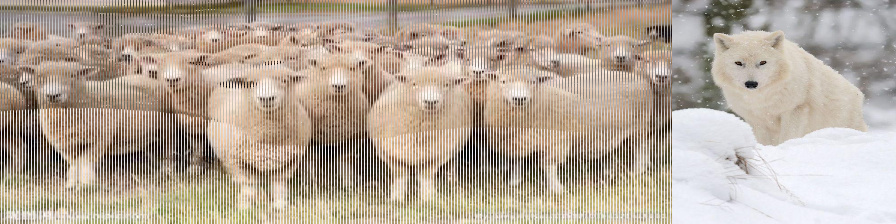
\includegraphics[width=\textwidth]{teaser.png}
  \caption{\DIFdelbegin \DIFdel{Illustration of }\DIFdelend \DIFaddbegin \DIFadd{Demonstrating }\DIFaddend an attack image \DIFdelbegin \DIFdel{that originally shows sheep, but shows a wolf }\DIFdelend \DIFaddbegin \DIFadd{$A$ and the resulting output image $D$ }\DIFaddend after being down-scaled \DIFdelbegin \DIFdel{. Source }\DIFdelend \cite{camouflage}\DIFaddbegin \DIFadd{.}\DIFaddend }
  \label{fig:teaser}
\end{teaserfigure}

%%
%% This command processes the author and affiliation and title
%% information and builds the first part of the formatted document.
\maketitle

\section{Introduction}
Within the last years, machine learning based applications have achieved remarkable success in lots of different application domains.
One very popular domain is computer vision, where especially the usage of convolutional neural networks results in applications that, in some benchmarks, even can beat human performance.
Since convolutional neural networks provide \DIFdelbegin \DIFdel{state of the art }\DIFdelend \DIFaddbegin \DIFadd{state-of-the-art }\DIFaddend prediction results in lots of different scenarios, also security critical applications may rely on them.
Examples for such applications are self-driving \DIFdelbegin \DIFdel{driving }\DIFdelend cars, biometric authentication systems or surveillance systems.

Besides the obvious benefits of machine learning based applications, these technologies also offer a new attack surface for adversaries.
\DIFdelbegin \DIFdel{Especially the }\DIFdelend \DIFaddbegin \DIFadd{The }\DIFaddend fact that machine learning algorithms often are treated as black-boxes makes them susceptible for new kinds of attacks.
That's why the security of such systems is a hot topic in current research.
Two very popular attacks on machine learning models that already have received lots of attention are evasion attacks\DIFdelbegin \DIFdel{aka adversarial examples}\DIFdelend \DIFaddbegin \DIFadd{, which commonly are applied by using adversarial examples, }\DIFaddend and poisoning attacks.
While evasion attacks aim to \DIFdelbegin \DIFdel{abuse }\DIFdelend \DIFaddbegin \DIFadd{exploit }\DIFaddend the test stage of a machine learning pipeline, poison attacks try to manipulate the attacked model at the training stage by inserting malicious training data.

Recently a new kind of attack has been demonstrated by Xiao et al.\cite{camouflage} which can be used to attack potentially any kind of application that involves image processing, i.e. image scaling, including image based machine learning models.
The new attack is called image-scaling attack and is applied at the preprocessing stage of the application's processing pipeline.
The key idea of this attack is to manipulate an image in a way that its visual appearance stays similar to the original image, but is completely changed after being down-scaled.
After Xiao et al.\DIFaddbegin \DIFadd{\mbox{%DIFAUXCMD
\cite{camouflage} }\hspace{0pt}%DIFAUXCMD
}\DIFaddend presented the attack, Quiring et al.\DIFaddbegin \DIFadd{\mbox{%DIFAUXCMD
\cite{imgscale} }\hspace{0pt}%DIFAUXCMD
}\DIFaddend further analyzed its root-cause and investigated the scaling algorithm implementations of the commonly used machine learning frameworks TensorFlow, Caffe and PyTorch.
Furthermore they showed that the attack can either be used in a similar way to evasion attacks or to support poisoning attacks \DIFdelbegin \DIFdel{\mbox{%DIFAUXCMD
\cite{imgscale, imgscalepoison}}\hspace{0pt}%DIFAUXCMD
}\DIFdelend \DIFaddbegin \DIFadd{\mbox{%DIFAUXCMD
\cite{imgscalepoison}}\hspace{0pt}%DIFAUXCMD
}\DIFaddend .
In addition they presented a proper defense that can sanitize an attacked image.

This report \DIFaddbegin \DIFadd{gives an overview about current research in the field of adversarial preprocessing with respect to the domain of computer vision.
Since we couldn't find any works about other attacks (within the domain of computer vision) that explicitly attack the preprocessing stage of a machine learning pipeline, we mainly focus on image-scaling attacks.
Thus, the report }\DIFaddend summarizes the new phenomenon of image-scaling attacks and recaps the key results from Quiring et al. and Xiao et al.\DIFaddbegin \DIFadd{\mbox{%DIFAUXCMD
\cite{imgscale, imgscalepoison, camouflage}}\hspace{0pt}%DIFAUXCMD
.
}\DIFaddend Therefore an introduction into image preprocessing in general as well as a background on evasion attacks and poisoning attacks is presented.
Furthermore the concept of the image-scaling attack is explained.
The methodology section of this work covers the concepts of creating an attack-image for an image-scaling attack as well as the root-cause that enables these attacks.
In addition possible mitigation strategies, i.e. detection methods \cite{camouflage} and defensive methods \cite{imgscale}, are described.
Following on that, it is briefly explained, how evasion-similar attacks and poisoning attacks can be \DIFdelbegin \DIFdel{achieved}\DIFdelend \DIFaddbegin \DIFadd{applied, using an image-scaling attack}\DIFaddend .
The experiments section briefly covers some of the experimental results of Quiring et al. and presents a few own experiments, based on their provided open source algorithms.
Finally a conclusion on image-scaling attacks is drawn.

\section{Background \DIFaddbegin \DIFadd{\& Related Work}\DIFaddend }
This section introduces the different domains which are related to the scope of image-scaling attacks.
At first, a brief overview on different preprocessing steps in deep learning pipelines, focusing on image scaling, is given.
\DIFdelbegin \DIFdel{Then the principle of image-scaling attacks is explained.
}\DIFdelend To give a further understanding of adversarial machine learning and how image-scaling attacks can be applied, evasion attacks as well as poisoning attacks are explained.

\subsection{Preprocessing and Image Scaling in Machine Learning}
\label{sec:prepimgscale}
In order to optimize and clean up the data that is put into a machine learning model, it is mandatory to preprocess the captured sensor signal that should be processed.
In the field of image processing such steps may be scaling, cropping, filtering and applying different affine transformations.
For example Taigman et al.\cite{6909616} use a complex alignment pipeline, including cropping and affine transformations to extract and frontalize a face from an image which then is used as input for their convolutional neural network. 

As the state of the art for image processing applications is based on convolutional neural networks (CNN) which \DIFaddbegin \DIFadd{generally }\DIFaddend require a fixed sized input, \DIFdelbegin \DIFdel{due to their convolutional layers, }\DIFdelend image scaling has become mandatory for such applications.
\DIFdelbegin \DIFdel{Since the amount of parameters of a CNN is affected by the size of the input image, the training and classification speed can be reduced by reducing the size of the input image.
Thus images often are downscaled to obtain a smaller sized image.
Note that images mostly are captured in high resolution.
}\DIFdelend This is even more amplified by the fact that it is a common practice to involve pretrained models in the training process of a \DIFdelbegin \DIFdel{convolutional neural network}\DIFdelend \DIFaddbegin \DIFadd{CNN}\DIFaddend .
Xiao et al.\cite{camouflage} reported input image sizes between $32 \times 32$ pixel and $299 \times 299$ for nine popular deep learning models.
\DIFaddbegin \DIFadd{Since images mostly are captured in a higher resolution, they are often down scaled to fit the input size of the used model.
}\DIFaddend 

This omnipresent usage of down-scaling for image processing applications results in a perfect base for the image-scaling attack which \DIFdelbegin \DIFdel{abuses }\DIFdelend \DIFaddbegin \DIFadd{exploits }\DIFaddend the implementation of downscaling algorithms.

There exist multiple different algorithms to down-scale an image which share the same goal and principles.
In general such an \DIFdelbegin \DIFdel{algorithms }\DIFdelend \DIFaddbegin \DIFadd{algorithm }\DIFaddend aims to reduce the original size $m \times n$ of an image to the new size $m' \times n$' while preserving the visual features of the image so that it looks similar to a human before and after the scaling process.
This is achieved by interpolating the pixels of the source image.
Each pixel of the down-scaled image is calculated by a weighted sum of its surrounding pixels.
The exact choice and weighting of the considered pixels is determined by the underlying algorithm.
Common algorithms for example are \DIFdelbegin \DIFdel{nearest neighbor }\DIFdelend \DIFaddbegin \DIFadd{nearest-neighbor }\DIFaddend or bilinear downscaling.
The concept of downscaling is illustrated in figure~\ref{fig:scaling}.

\begin{figure}[h]
  \centering
  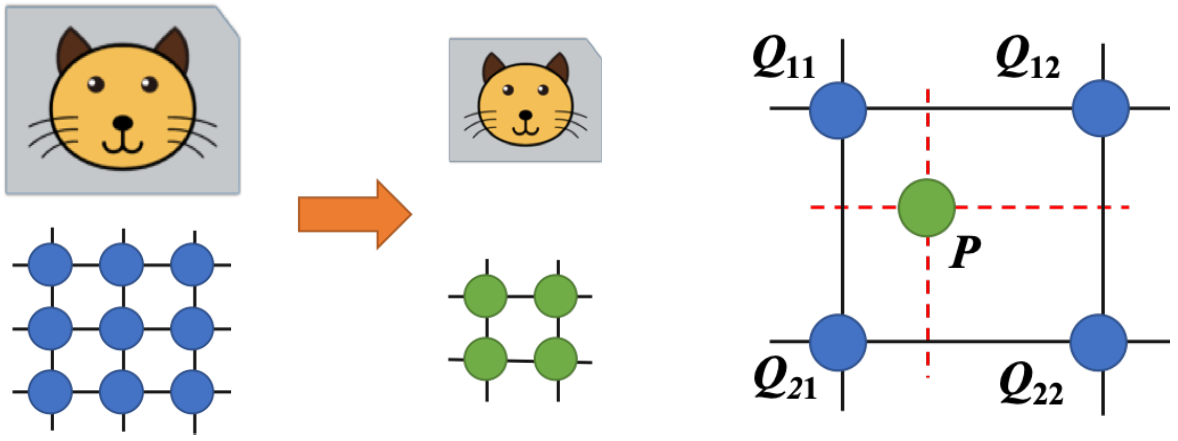
\includegraphics[width=\linewidth]{img/img_scaling.png}
  \caption{\DIFdelbeginFL \DIFdelFL{Concept }\DIFdelendFL \DIFaddbeginFL \DIFaddFL{Demonstrating the concept }\DIFaddendFL of image downscaling. \DIFdelbeginFL \DIFdelFL{Source }\DIFdelendFL \DIFaddbeginFL \DIFaddFL{The pixels $Q_{11}$, $Q_{12}$, $Q_{21}$, $Q_{22}$ of the original image are interpolated to gain the new pixel value $P$ of the down-scaled image }\DIFaddendFL \cite{camouflage}\DIFaddbeginFL \DIFaddFL{.}\DIFaddendFL }
  \Description{}
  \label{fig:scaling}
\end{figure}

Since downscaling is a mandatory step for image preprocessing, common deep learning frameworks like TensorFlow, Caffe and PyTorch support different downscaling algorithms such as nearest-neighbor-, bilinear-, bicubic- and area-downscaling.
According to Quiring et al.\cite{imgscale} other deep learning libraries are either based on the mentioned frameworks or on OpenCV and Pillow which also is the base for Caffe and PyTorch.
Thus the availability of different downscaling algorithms is limited to a few implementations which makes it easy for an attacker to guess the image scaling algorithm in a \DIFdelbegin \DIFdel{black-box scenario .
}%DIFDELCMD < 

%DIFDELCMD < %%%
\subsection{\DIFdel{Image-Scaling Attacks}}
%DIFAUXCMD
\addtocounter{subsection}{-1}%DIFAUXCMD
%DIFDELCMD < \label{sec:imgscaleattack}
%DIFDELCMD < %%%
\DIFdel{The goal of an image-scaling attack is to manipulate a source image, which might serve as input for an image processing model, in a way, that its appearance and thus its semantic changes when it is processed by a downscaling algorithm.
This means that the attacker tries to break the property of a downscaling algorithm that the visual features of the down-scaled image are preserved.
One major constraint on such an image-scaling attack is , that the manipulated image has to be similar to the original source image in order to make the attack hardly visible for a human observer.
}%DIFDELCMD < 

%DIFDELCMD < \begin{figure}[h]
%DIFDELCMD <   \centering
%DIFDELCMD <   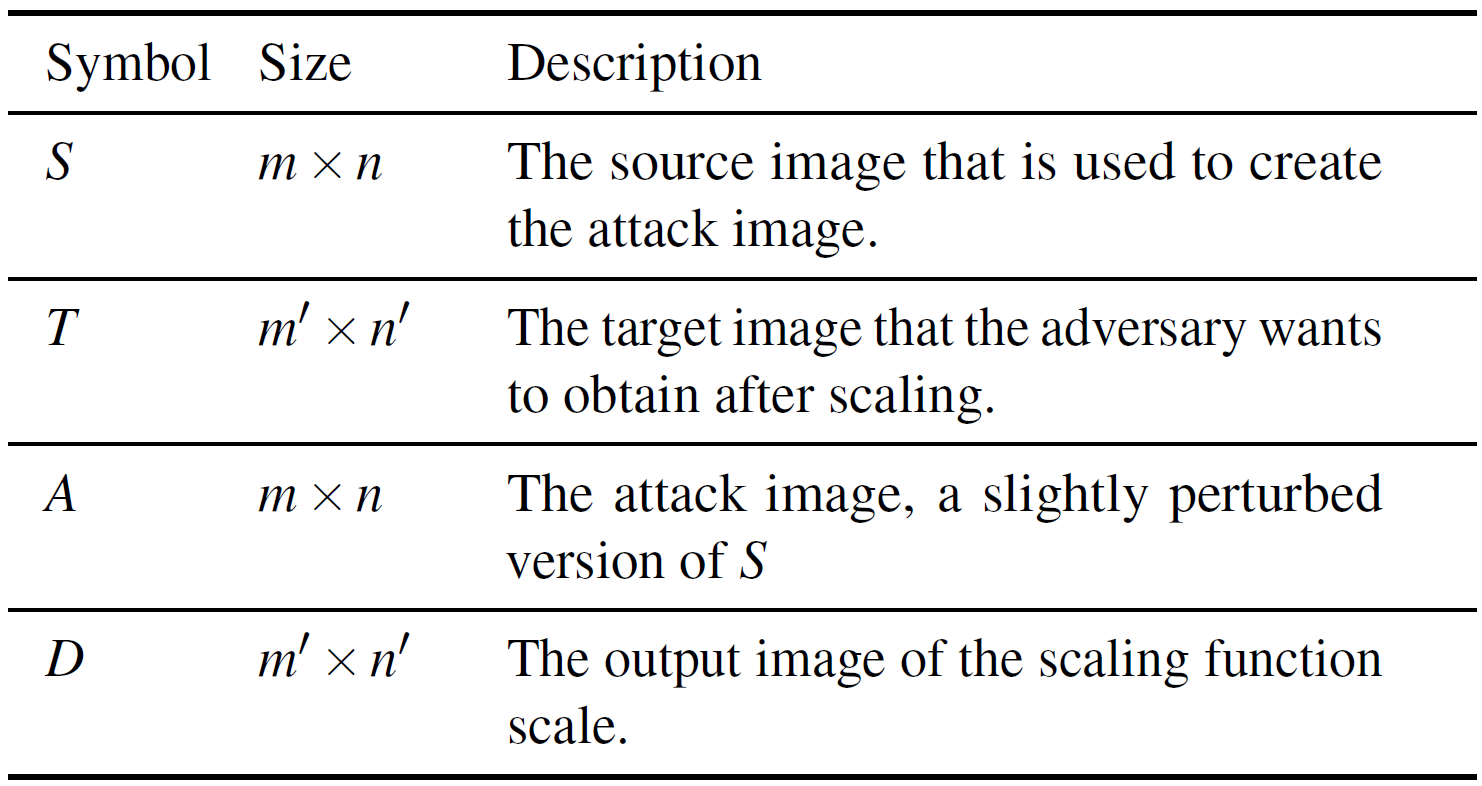
\includegraphics[width=\linewidth]{img/table_attack_symbols.png}
%DIFDELCMD <   %%%
%DIFDELCMD < \caption{%
{%DIFAUXCMD
\DIFdelFL{Major Objects of an Image-Scaling Attack. Source \mbox{%DIFAUXCMD
\cite{imgscale}}\hspace{0pt}%DIFAUXCMD
}}
  %DIFAUXCMD
%DIFDELCMD < \Description{}
%DIFDELCMD <   %DIFDELCMD < \label{fig:table}%%%
%DIFDELCMD < \end{figure}
%DIFDELCMD < 

%DIFDELCMD < %%%
\DIFdel{Formally there are four major objects to consider for an image-scaling attack, shown in figure~\ref{fig:table}.
In order to perform the attack, the attacker first crafts the attack image $A$ by carefully manipulating key pixels of the source image $S$.
Then he replaces $A$ with $S$ so that the scaling procedure of the image processing pipeline is applied to $A$.
This process is illustrated in figure \ref{fig:conc}.
In the case of a successful attack, the output image $O$ looks similar to the target image $T$ while the attack image $A$ looks similar to the source image $S$.
These two conditions can be seen as the main Objectives of an image-scaling attack and can be formalized as:
$\boldsymbol{O_1}$) $scale(A) \sim T$ and $\boldsymbol{O_2}$) $A \sim S$}\DIFdelend \DIFaddbegin \DIFadd{scenario where no explicit knowledge about the used algorithm is given}\DIFaddend .

\DIFdelbegin %DIFDELCMD < \begin{figure}[h]
%DIFDELCMD <   \centering
%DIFDELCMD <   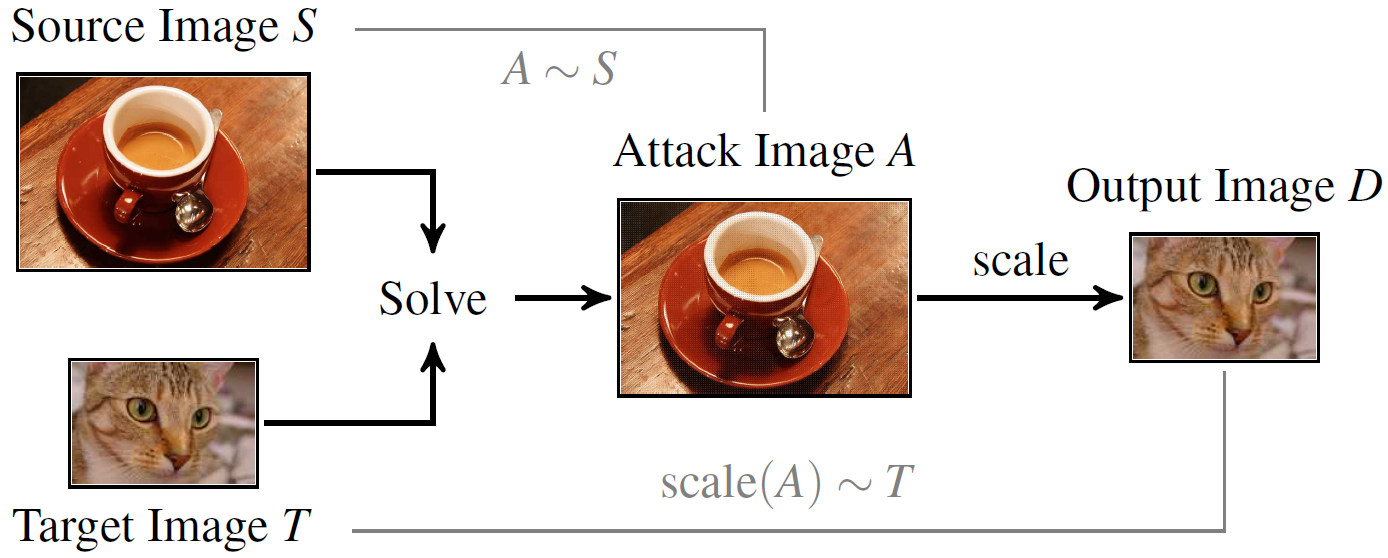
\includegraphics[width=\linewidth]{img/img_scale_concept.png}
%DIFDELCMD <   %%%
%DIFDELCMD < \caption{%
{%DIFAUXCMD
\DIFdelFL{Concept of the Image-Scaling Attack. Source \mbox{%DIFAUXCMD
\cite{imgscale}}\hspace{0pt}%DIFAUXCMD
}}
  %DIFAUXCMD
%DIFDELCMD < \Description{}
%DIFDELCMD <   %DIFDELCMD < \label{fig:conc}%%%
%DIFDELCMD < \end{figure}
%DIFDELCMD < 

%DIFDELCMD < %%%
\DIFdel{According to Xiao et al.\mbox{%DIFAUXCMD
\cite{camouflage} }\hspace{0pt}%DIFAUXCMD
an image-scaling attack can be performed in two attack modes which are called weak attack mode and and strong attack mode.
While the attacker is allowed to specify the source image S as well as the target image T in the strong attack mode, the weak attack mode only allows to choose the target image T, while S is fixed.
}%DIFDELCMD < 

%DIFDELCMD < %%%
\DIFdel{Since an image-scaling attack is performed within the preprocessing stage of an image processing pipeline, which is located before the feature extraction stage, it can effect all subsequent stages.
In the case of deep learning model this especially includes the training as well as the testing stage.
This makes it possible for an attacker to either execute cloaked poisoning attacks by adding malicious data to the training data set or executing attacks }\DIFdelend \DIFaddbegin \subsection{\DIFadd{Evasion Attacks}}
\DIFadd{The term evasion attacks commonly describes attacks against machine learning models that are performed }\DIFaddend at test time\DIFdelbegin \DIFdel{by manipulating the tested input image.
Furthermore an image-scaling attack is independent from the attacked model itself and thus can be applied without any knowledge of the attacked model.
Even image processing applications that do not use machine learning models might suffer from }\DIFdelend \DIFaddbegin \DIFadd{.
The goal of }\DIFaddend such an attack \DIFdelbegin \DIFdel{.
}%DIFDELCMD < 

%DIFDELCMD < %%%
\DIFdel{Considering the required knowledge of an attacker, Xiao et al. showed that it is possible to perform white-box as well as black-box scaling attacks.
There are only two things an attacker must know:
 }\textbf{\DIFdel{a)}} %DIFAUXCMD
\DIFdel{the used scaling algorithm
 }\textbf{\DIFdel{b)}} %DIFAUXCMD
\DIFdel{the size of the scaled image.
In a white-box scenarios these information are present per definition.
In a black-box scenario Xiao et al. showed that the attacker is able to infer the required knowledge using an exhaustive search were they send a series of probing images, ``crafted by the scaling method with various scaling parameters`` (see \mbox{%DIFAUXCMD
\cite{camouflage}}\hspace{0pt}%DIFAUXCMD
) to }\DIFdelend \DIFaddbegin \DIFadd{is to produce false prediction results of }\DIFaddend the attacked model \DIFdelbegin \DIFdel{and observe the classification result.
This especially is possible due to the limited potential options for the scaling algorithms, as mentioned before.
In their work they additionally describe an optimized approach that can retrieve the desired information more efficiently.
}%DIFDELCMD < 

%DIFDELCMD < %%%
\DIFdel{As mentioned above, image scaling is only one of many possible preprocessing steps that might be performed within an image processing pipeline.
Depending on the kind of preprocessing steps and their ordering within the pipeline, they can interfere with the image scaling attack.
If an image for example is first rotated and then scaled, the image scaling attack probably won't work anymore, since the carefully manipulated pixels changed their location and thus their effect on the scaling algorithm.
However such interference can be bypassed, if the attacker knows about them, by considering them in her attack.
}%DIFDELCMD < 

%DIFDELCMD < %%%
\subsection{\DIFdel{Evasion Attacks}}
%DIFAUXCMD
\addtocounter{subsection}{-1}%DIFAUXCMD
\DIFdel{Evasion attacks which are also known as adversarial examplesare quite similar to image-scaling attacks at test time.
One major difference to these attacks is, that adversarial examples are specifically crafted to fool one specific deep learning model at test time instead of attacking the preprocessing stage and thus being model independent.
This can be achieved }\DIFdelend \DIFaddbegin \DIFadd{for specific inputs.
In general these specific inputs are adversarial examples.
An adversarial example is a precisely manipulated model input that can be created, }\DIFaddend by applying small perturbations to the original input\DIFdelbegin \DIFdel{image of a deep learning model (the attacked model) so that the resulting image is missclassified by }\DIFdelend \DIFaddbegin \DIFadd{.
Therefore the perturbations are calculated in respect to }\DIFaddend the attacked model\DIFdelbegin \DIFdel{.
Note that the intended behavior of model }\DIFdelend \DIFaddbegin \DIFadd{, a surrogate model or a specific data set.
While the attacked model creates wrong predictions, if an adversarial example is given, its intended behavior }\DIFaddend under normal circumstances is not influenced.

\DIFdelbegin %DIFDELCMD < \begin{figure}[h]
%DIFDELCMD <   \centering
%DIFDELCMD <   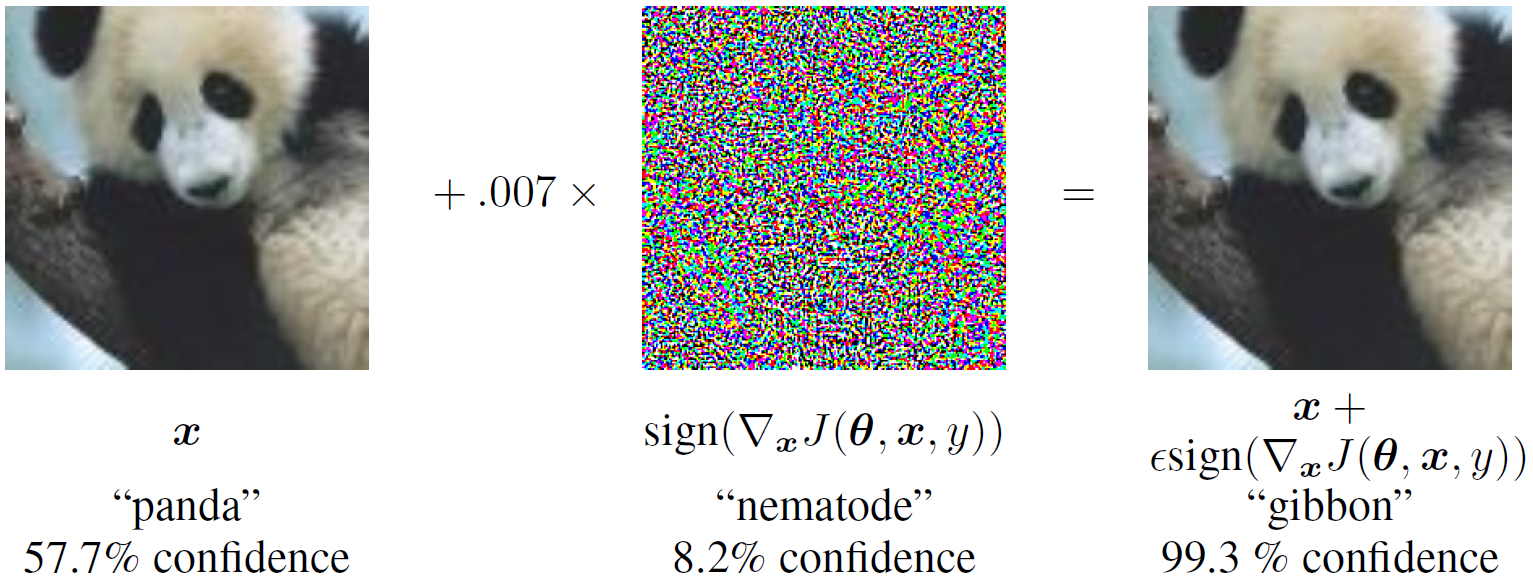
\includegraphics[width=\linewidth]{img/advex.png}
%DIFDELCMD <   %%%
%DIFDELCMD < \caption{%
{%DIFAUXCMD
\DIFdelFL{Illustration of an adversarial example. Source \mbox{%DIFAUXCMD
\cite{43405}}\hspace{0pt}%DIFAUXCMD
}}
  %DIFAUXCMD
%DIFDELCMD < \Description{}
%DIFDELCMD < \end{figure}
%DIFDELCMD < 

%DIFDELCMD < %%%
\DIFdelend In contrast to adversarial preprocessing, adversarial examples have seen lots of attention within the last years.
Firstly the concept of adversarial examples was reported by Szegedy et al.\cite{intr}.
In their work, they called them intriguing properties and showed that these properties are non-random and can be applied to multiple different deep learning models.
In a following work, Goodfellow et al.\cite{43405} presented a more detailed analyze of adversarial examples and explained that the root-cause of adversarial examples is that most deep learning models are too linear.
Furthermore they presented a simple and fast method to generate such examples called \DIFdelbegin \DIFdel{``fast gradient sign method``}\DIFdelend \DIFaddbegin \textit{\DIFadd{fast gradient sign method}}\DIFaddend .

Since this method directly calculates the required gradients and assumes the knowledge of the used cost function of the attacked model, this method can be seen as a white-box attack \DIFaddbegin \DIFadd{(an attack with full knowledge about the used model, algorithms and other relevant details)}\DIFaddend .
One early example of an attack with adversarial examples was presented by Kurakin et al.\cite{advexinphys}.
In 2016 Papernot et al.\cite{Papernot2017PracticalBA} showed that it is also possible to perform black-box attacks \DIFaddbegin \DIFadd{(attacks with limited knowledge about the used model, algorithms etc.) }\DIFaddend with adversarial examples.
This could be achieved by creating a \DIFdelbegin \DIFdel{substitute }\DIFdelend \DIFaddbegin \DIFadd{surrogate }\DIFaddend model which mimics the attacked model and is used to generate the adversarial examples. 
\DIFdelbegin \DIFdel{Other interesting works in the field of adversarial examples are \mbox{%DIFAUXCMD
\cite{8578273, brown2018adversarial, 10.1007/978-3-642-40994-3_25}}\hspace{0pt}%DIFAUXCMD
.
}\DIFdelend \DIFaddbegin \DIFadd{~}\footnote{\DIFadd{Other interesting works in the field of adversarial examples are \mbox{%DIFAUXCMD
\cite{8578273, brown2018adversarial, 10.1007/978-3-642-40994-3_25}}\hspace{0pt}%DIFAUXCMD
. However, they are not required to understand this report and thus are not further explained.}}
\DIFaddend 

Besides developing different evasion attacks, there also has been research towards defenses against such attacks.
One potential defense which involves a second model, that is trained to predict the input of another model and thus learns soft labels instead of hard labels, was presented by Papernot et al.\cite{7546524}.
However even though they showed, that this so called defensive distillation could reduce the effectiveness of an adversarial attack by a lot for a specific deep learning model, it turned out, that the approach does not provide proper protection against advanced evasion attack strategies.
This was proven by Papernot et al.\cite{Papernot2017PracticalBA} as well as Carlini \& Wagner\cite{7958570}.
\DIFdelbegin \DIFdel{Other works that observe defense strategies against adversarial examples for example are \mbox{%DIFAUXCMD
\cite{8835364, madry2019deep}}\hspace{0pt}%DIFAUXCMD
.
}\DIFdelend \DIFaddbegin \DIFadd{~}\footnote{\DIFadd{Other works that observe defense strategies against adversarial examples for example are \mbox{%DIFAUXCMD
\cite{8835364, madry2019deep}}\hspace{0pt}%DIFAUXCMD
.}}
\DIFaddend 

\subsection{Poisoning Attacks}
\label{sec:poison}

In general poisoning attacks aim to manipulate the training data or their labels of a machine learning model to ultimately change the model's behavior at test time.
There are two types of poisoning attacks that can be distinguished: non-targeted attacks and targeted attacks.
While non-targeted attacks simply try to force the attacked model to misbehave, targeted attacks aim to make the model sensible for specific input patterns.

\DIFdelbegin %DIFDELCMD < \begin{figure}[h]
%DIFDELCMD <   \centering
%DIFDELCMD <   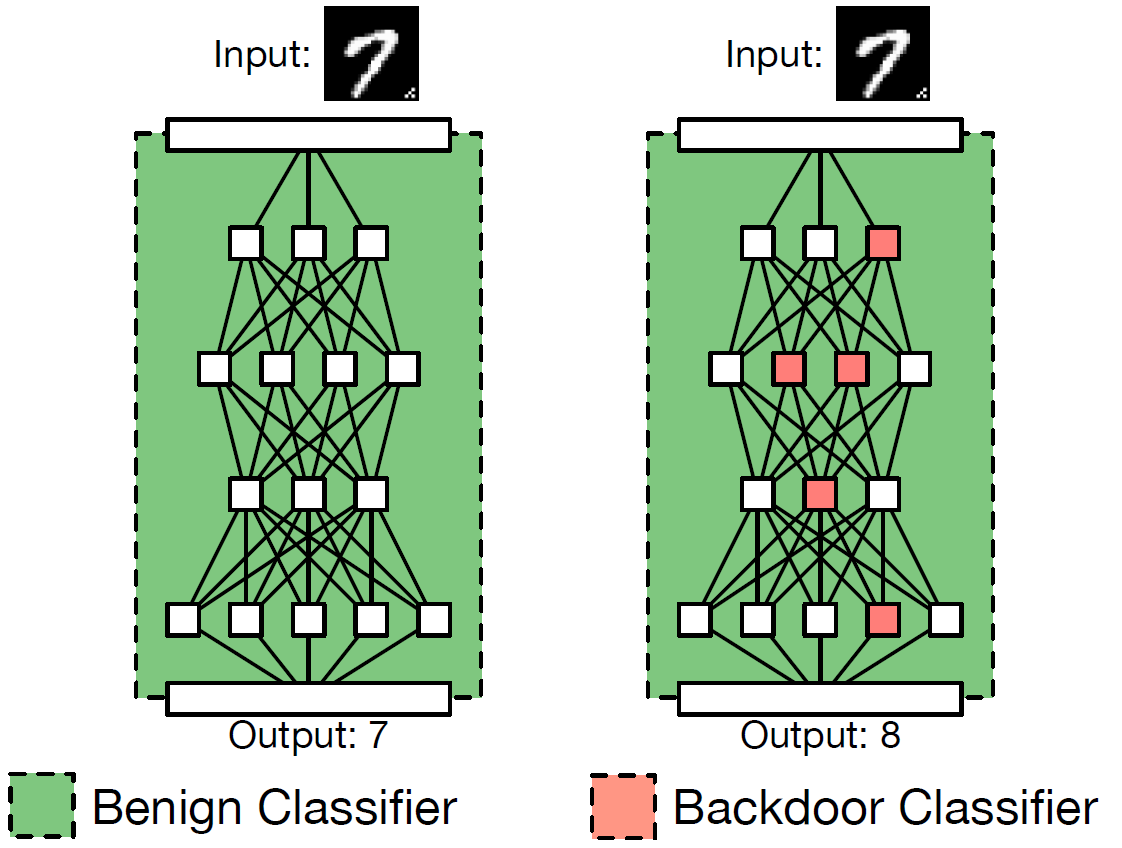
\includegraphics[width=\linewidth]{img/badnet.png}
%DIFDELCMD <   %%%
%DIFDELCMD < \caption{%
{%DIFAUXCMD
\DIFdelFL{Illustration of backdooring a neural network. Source \mbox{%DIFAUXCMD
\cite{8685687}}\hspace{0pt}%DIFAUXCMD
}}
  %DIFAUXCMD
%DIFDELCMD < \Description{``Approaches to backdooring a neural network. On the left, a clean network correctly classifies its input. An attacker could ideally use a separate
%DIFDELCMD < network (center) to recognize the backdoor trigger, but is not allowed to change the network architecture. Thus, the attacker must incorporate the backdoor
%DIFDELCMD < into the user-specified network architecture (right).``}
%DIFDELCMD < \end{figure}
%DIFDELCMD < 

%DIFDELCMD < %%%
\DIFdelend An early approach on poisoning a machine learning model was reported by Biggio et al.\cite{svmPoison}.
In their work they investigated the model's behavior under the attack of an adversary that could flip a subset of the labels of the training data and proposed a method to make the SVM more robust against this kind of attack.

One of the first poisoning attack against deep learning models was proposed by Muñoz-González et al.\cite{DBLP:journals/corr/abs-1708-08689}.
Until then, the computational power that was needed to optimize the poisoning points (instead of arbitrarily changing the data or labels) was too high to effectively be applied in attack scenarios.
Their proposed poisoning algorithm, called back-gradient optimization, greatly reduced the computational complexity and thus was feasible to be applied to deep learning models such as CNNs. 
Due to the usage of a surrogate learner, they also showed, that a poisoning attack can be applied with limited knowledge and thus be applicable in a black-box setting.
Another interesting work to mention, which applied an poisoning attack on deep learning models is \cite{koh2017understanding}.

An approach of a targeted poisoning attack is given by Liu et al.\cite{trojanattack}.
They introduced the trojaning attack on neural networks which is used to install a trojan trigger into the network.
Such a trigger can be a small, specifically engineered patch of pixels on an image.
The trigger installation is not directly applied at the train time of the model.
Moreover, Liu et al. propose a retrain mechanism that can be applied after the model was trained and thus requires much less computational effort than an attack that happens at train time.
When retraining the model, it learns a specified malicious behavior (i.e. targeted misclassifications) which finally will be triggered on test time, as soon as an image with the trigger on it is used as input image.

Another targeted poisoning attack on deep learning models that can be triggered on specific patterns or inputs was shown by Gu et al.\cite{8685687}.
They called the networks that are affected by such an attack BadNets and described a realistic scenario of attacking a street sign classifier to ultimately predict stop signs as speed limits, whenever a special sticker is added to a stop sign.
Note that BadNets obtain the capability to do correct predictions in normal circumstances, i.e. if no trigger pattern is present.

Shafahi et al.\cite{10.5555/3327345.3327509} introduced a new kind of targeted poisoning attacks which they call clean-label poisoning attack.
Such an attack can be performed without actually having control over the labeling or training data.
\DIFdelbegin %DIFDELCMD < 

%DIFDELCMD < %%%
\DIFdel{Potential defenses against poisoning attacks for example are handled in \mbox{%DIFAUXCMD
\cite{neuralCleanse, DBLP:journals/corr/abs-1905-13409}}\hspace{0pt}%DIFAUXCMD
.
}\DIFdelend \DIFaddbegin \DIFadd{~}\footnote{\DIFadd{Potential defenses against poisoning attacks for example are handled in \mbox{%DIFAUXCMD
\cite{neuralCleanse, DBLP:journals/corr/abs-1905-13409}}\hspace{0pt}%DIFAUXCMD
.}}
\DIFaddend 

\section{\DIFdelbegin \DIFdel{Methodology}\DIFdelend \DIFaddbegin \DIFadd{Image-Scaling Attacks}\DIFaddend }
This section explains \DIFdelbegin \DIFdel{how }\DIFdelend \DIFaddbegin \DIFadd{the principles of }\DIFaddend image-scaling attacks\DIFdelbegin \DIFdel{work in more detail.
First }\DIFdelend \DIFaddbegin \DIFadd{.
After formally introducing the attack, }\DIFaddend it is described, how an attack image automatically can be created solving an optimization problem.
To simplify things, only the strong attack \DIFaddbegin \DIFadd{(see section~\ref{sec:imgscaleattack})}\DIFaddend , which is the more realistic one, is explained.
Following on that, the root-cause that enables image-scaling attacks is presented.
Furthermore the possibilities of using an image-scaling attack for attacks at test and train time as well as defense strategies against these attacks are explained.

\subsection{Image-Scaling Attack \DIFaddbegin \DIFadd{Introduction}\DIFaddend }
\DIFaddbegin \label{sec:imgscaleattack}
\DIFadd{The goal of an image-scaling attack is to manipulate a source image, which might serve as input for an image processing model, in a way, that its appearance and thus its semantic changes when it is processed by a downscaling algorithm.
This means that the attacker tries to break the property of a downscaling algorithm that the visual features of the down-scaled image are preserved.
One major constraint on such an image-scaling attack is, that the manipulated image has to be similar to the original source image in order to make the attack hardly visible for a human observer.
}

\begin{figure}[h]
  \centering
  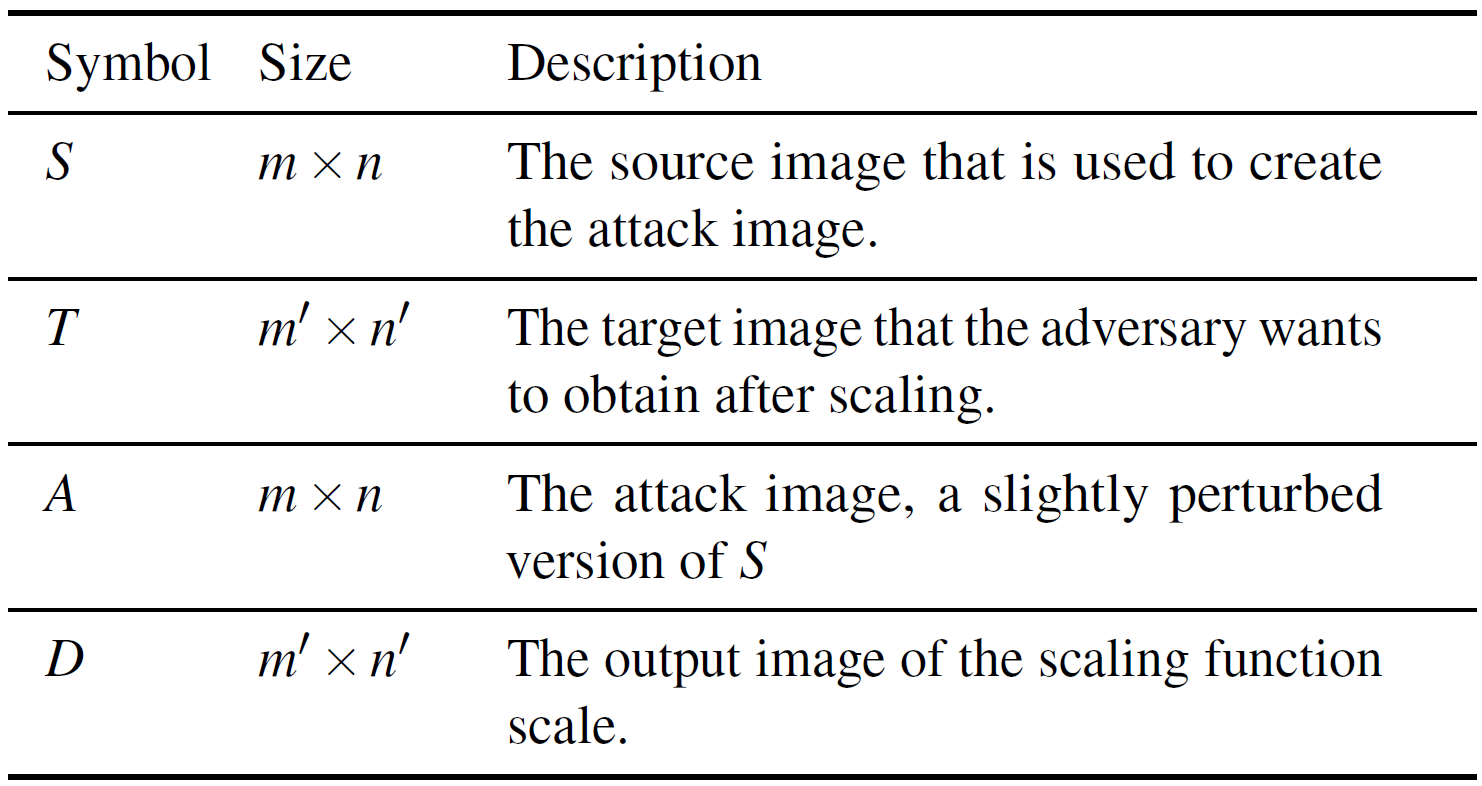
\includegraphics[width=\linewidth]{img/table_attack_symbols.png}
  \caption{\DIFaddFL{Showing the major objects of an image-scaling attack \mbox{%DIFAUXCMD
\cite{imgscale}}\hspace{0pt}%DIFAUXCMD
.}}
  \Description{}
  \label{fig:table}
\end{figure}

\DIFadd{Formally there are four major objects to consider for an image-scaling attack, shown in figure~\ref{fig:table}.
In order to perform the attack, the attacker first crafts the attack image $A$ by carefully manipulating key pixels of the source image $S$ in respect to the target image $T$.
Then $S$ is replaced by $A$ so that the scaling procedure $scale()$ of the image processing pipeline is applied to $A$.
In the case of a successful attack, the output image $D$ looks similar to the target image $T$ while the attack image $A$ looks similar to the source image $S$.
These two conditions can be seen as the main objectives of an image-scaling attack and can be formalized as:
}

\begin{equation}
\DIFadd{\label{eq:O1}
\boldsymbol{O_1})~scale(A) \sim T
}\end{equation}
\begin{equation}
\DIFadd{\label{eq:O2}
\boldsymbol{O_2})~A \sim S
}\end{equation}

\DIFadd{Here $\sim$ expresses similarity between the two operands.
}

\DIFadd{In figure \ref{fig:conc} the described concept of an image-scaling attack is demonstrated.
Furthermore an example of a potential attack image $A$ and its corresponding output image $D$ is shown in figure \ref{fig:teaser}.
The left image of the figure, which is the attack image $A$, clearly shows sheep, while the right image, the output image $D$, perfectly shows a wolf.
}

\begin{figure}[h]
  \centering
  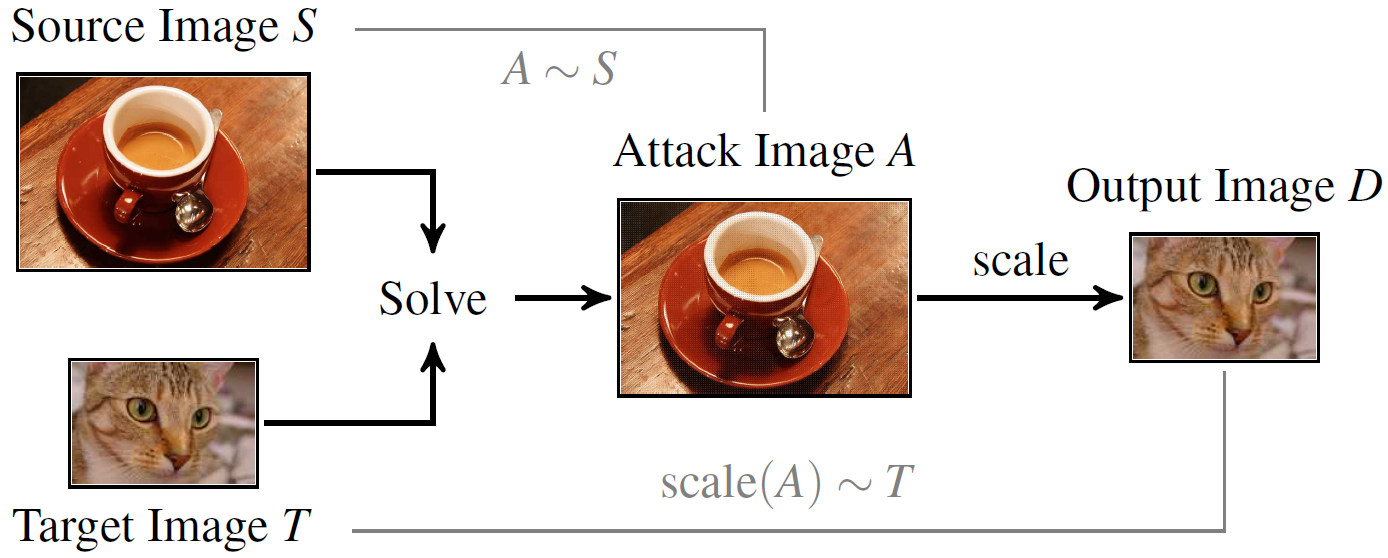
\includegraphics[width=\linewidth]{img/img_scale_concept.png}
  \caption{\DIFaddFL{Demonstrating the concept of an image-scaling attack \mbox{%DIFAUXCMD
\cite{imgscale}}\hspace{0pt}%DIFAUXCMD
.}}
  \Description{}
  \label{fig:conc}
\end{figure}

\DIFadd{According to Xiao et al.\mbox{%DIFAUXCMD
\cite{camouflage} }\hspace{0pt}%DIFAUXCMD
an image-scaling attack can be performed in two attack modes which are called weak attack mode and strong attack mode.
While the attacker is allowed to specify the source image $S$ as well as the target image $T$ in the strong attack mode, the weak attack mode only allows to choose the target image $T$, while $S$ is fixed.
}

\DIFadd{Since an image-scaling attack is performed within the preprocessing stage of an image processing pipeline, which is located before the feature extraction stage, it can effect all subsequent stages.
In the case of a deep learning model this especially includes the training as well as the testing stage.
This makes it possible for an attacker to either execute cloaked poisoning attacks by adding malicious data to the training data set or executing attacks at test time by manipulating the tested input image.
Furthermore an image-scaling attack is independent from the attacked model itself and thus can be applied without any knowledge of the attacked model.
Even image processing applications that do not use machine learning models might suffer from such an attack.
}

\DIFadd{Considering the required knowledge of an attacker, Xiao et al. showed that it is possible to perform white-box  as well as black-box scaling attacks.
There are only two things an attacker must know:
 }\textbf{\DIFadd{a)}} \DIFadd{the used scaling algorithm
 }\textbf{\DIFadd{b)}} \DIFadd{the size of the scaled image.
In a white-box scenario these information are present per definition.
In a black-box scenario Xiao et al. showed that the attacker is able to infer the required knowledge using an exhaustive search where they send a series of probing images, ``crafted by the scaling method with various scaling parameters`` (see \mbox{%DIFAUXCMD
\cite{camouflage}}\hspace{0pt}%DIFAUXCMD
) to the attacked model and observe the classification result.
This especially is possible due to the limited potential options for the scaling algorithms, as mentioned before.
In their work they additionally describe an optimized approach that can retrieve the desired information more efficiently.
}

\DIFadd{As mentioned above, image scaling is only one of many possible preprocessing steps that might be performed within an image processing pipeline.
Depending on the kind of preprocessing steps and their ordering within the pipeline, they can interfere with the image scaling attack.
If an image for example is first rotated and then scaled, the image scaling attack probably won't work anymore, since the carefully manipulated pixels changed their location and thus their effect on the scaling algorithm.
However such interference can be bypassed, if the attacker knows about them, by considering them in the attack.
}

\subsection{\DIFadd{Creating the Attack Image}}
\DIFaddend In order to perform an effective image-scaling attack it is mandatory to automatically and efficiently create a strong attack image $A$.
Mathematically the attack image $A$ can be created by adding a perturbation matrix ${\Delta}_1$ to the source image $S$: $A = S + {\Delta}_1$.
As described in section \ref{sec:imgscaleattack} the output image \DIFdelbegin \DIFdel{$O$ }\DIFdelend \DIFaddbegin \DIFadd{$D$ }\DIFaddend results by scaling the attack image $A$ with a certain scaling function $scale()$ which can be formalized as: \DIFdelbegin \DIFdel{$O = scale(A)$}\DIFdelend \DIFaddbegin \DIFadd{$D = scale(A)$}\DIFaddend .
Note that there exist multiple different possible $A_i$ that result in the same \DIFdelbegin \DIFdel{$O$}\DIFdelend \DIFaddbegin \DIFadd{$D$}\DIFaddend .
Thus the attacker wants to find the $A$ that satisfies $\boldsymbol{O_1}$ and $\boldsymbol{O_2}$\DIFdelbegin \DIFdel{mentioned in section \ref{sec:imgscaleattack} }\DIFdelend \DIFaddbegin \DIFadd{~(equations~\ref{eq:O1},~\ref{eq:O2}) }\DIFaddend the most.
The relation between \DIFdelbegin \DIFdel{$O$ }\DIFdelend \DIFaddbegin \DIFadd{$D$ }\DIFaddend and $T$, which is relevant for objective $\boldsymbol{O_1}$ is noted as follows: \DIFdelbegin \DIFdel{$O = {\Delta}_2$}\DIFdelend \DIFaddbegin \DIFadd{$D = T + {\Delta}_2$}\DIFaddend , where ${\Delta}_2$ is another perturbation matrix.
To measure the similarity between $A$ and $S$ as well as the similarity between \DIFdelbegin \DIFdel{$O$ }\DIFdelend \DIFaddbegin \DIFadd{$D$ }\DIFaddend and $T$, Xiao et al. have chosen the $L$-norm.
Putting all together, Xiao et al.\cite{camouflage} concluded that the optimal attack image $A$ can be created solving the following objective function: 
$$\min(\lVert{\Delta}_1\rVert ^2) {,~s.t.~} {\lVert{\Delta}_2\rVert}_\infty \leq \epsilon * {\mathbb{N}}_{max},$$
where ${\mathbb{N}}_{max}$ is the maximum pixel value in the current image format (e.g. 255 for 8-bit RGB images).

To solve this function in an efficient way, Xiao et al. make use of the fact, that all analyzed scaling algorithm performed the scaling in two steps: first reducing the horizontal dimension and then reducing the vertical dimension (or vice versa).
This results in the following equation for an arbitrary image $I$: $scale(I) = L~*~I~*~R$. where $L$ and $R$ are two fixed coefficient matrices with dimension $m' \times m$ and $n \times n'$ assuming dimension $m \times n$ of the scaled image $I$.
Note that $L$ and $R$ are determined by the used scaling algorithm and have to be calculated by the attacker.
Overall the relation between source and target image that is required to create the attack image is described by Xiao et al. by:
$$L~*~(S + {\Delta}_1)~*~R = \DIFdelbegin \DIFdel{O }\DIFdelend \DIFaddbegin \DIFadd{D }\DIFaddend $$
$$ \DIFdelbegin \DIFdel{O }\DIFdelend \DIFaddbegin \DIFadd{D }\DIFaddend = T +  {\Delta}_2$$

Finally Xiao et al. show that the attack image ultimately can be generated solving a convex optimization problem based on these equations.
\DIFdelbegin \DIFdel{Fore }\DIFdelend \DIFaddbegin \DIFadd{For }\DIFaddend more details and information on the slight differences between the weak and the strong attack see ~ \cite{camouflage}.

\subsection{Image-Scaling Attack Analysis}
\label{sec:imgscalemethod}
Quiring et al.\cite{imgscale} picked up the work of Xiao et al. and performed a deeper analysis of image-scaling attacks to understand the root-cause that enables such attacks.
At first Quiring et al. compared image-scaling to signal processing and argued that the information loss that happens on down-scaling can be regarded as the loss of certain frequencies of the image signal.
Thus the Nyquist-Shannon theorem \cite{10.5555/1795494} can be applied which says that the original signal, i.e. the original image $I$, can not unambiguously be reconstructed if the sampling rate is too low.
This effect, which is \DIFdelbegin \DIFdel{abused }\DIFdelend \DIFaddbegin \DIFadd{exploited }\DIFaddend by the attacker, is called \DIFdelbegin \DIFdel{called }\DIFdelend aliasing effect.

In the case of image scaling, the sampling of the original image $I$ is done by a convolution between $I$ and a kernel function.
Each pixel of the down-scaled image results from a weighted sum of a pixel subset of the original image.
Therefore the kernel function, which defines the weighting of the regarded pixels, is moved as a window over the image with a specific step size.
This procedure is done in order to minimize the aliasing effect when down-scaling an image.
However not every pixel regarded by the kernel function contributes equally to the down-scaling process and the step size of the kernel movement highly depends on the scaling ratio between $I$ and the scaled image $I'$.
Thus an attacker only has to manipulate the subset of pixels that have a big contribution to the scaling process and can disregard the other pixels.
Quiring et al. presented \DIFdelbegin \DIFdel{the following }\DIFdelend figure \ref{sec:conscale} to demonstrate such a convolution for horizontal scaling within a single row.
Note that this concept is transferable to the scaling of a whole image.

\begin{figure}[h]
  \centering
  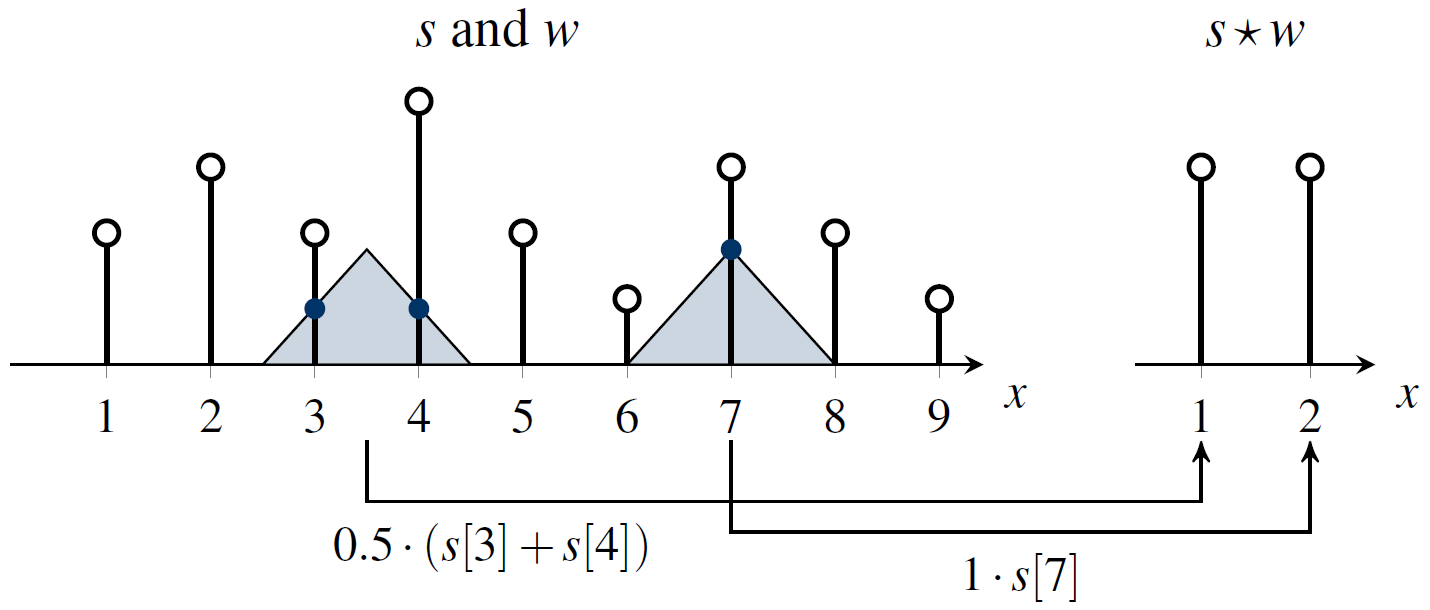
\includegraphics[width=\linewidth]{img/conscale.png}
  \caption{Illustration of a convolution \DIFdelbeginFL \DIFdelFL{for horizontal scaling}\DIFdelendFL \DIFaddbeginFL \DIFaddFL{of the signal $s$ with the kernel $w$}\DIFaddendFL . \DIFdelbeginFL \DIFdelFL{Source }\DIFdelendFL \DIFaddbeginFL \DIFaddFL{Only 3 out of 9 values of $s$ contribute to the resulting signal $s \star w$ }\DIFaddendFL \cite{imgscale}\DIFaddbeginFL \DIFaddFL{.}\DIFaddendFL }
  \Description{}
  \label{sec:conscale}
\end{figure}

Based on these insights, Quiring et al. identified two critical parameters that define the sparsity of the sampled pixels with high contribution, i.e. high weights, of the source image and thus \DIFdelbegin \DIFdel{effect }\DIFdelend \DIFaddbegin \DIFadd{affect }\DIFaddend the potential success of an attacker.
These are the scaling ratio $\beta$ which describes the size ratio between the original image $I$ and the scaled image $I'$ and the kernel width $\sigma$ which defines the size of the kernel window that is moved over the source image $I$.
Note that $\beta$ and $\sigma$ each can be separated in horizontal and a vertical component in case of a non-quadratic image: ${\beta}_h$, ${\beta}_v$, ${\sigma}_h$, ${\sigma}_v$.
While increasing the scaling ratio $\beta$ when $\sigma$ is fixed, increases the sparsity of pixels, the increase of $\sigma$ on a fixed $\beta$ works vice versa.
Thus a high $\beta$ and a small $\sigma$ result in a perfect attack surface for an attacker. 

Bringing all of this to a conclusion, the fact that potentially only a few subset of pixels of the original image $I$ are crucial for the down-scaling process, enables an attacker to perform an image-scaling attack that is \DIFdelbegin \DIFdel{hardly }\DIFdelend \DIFaddbegin \DIFadd{hard }\DIFaddend to detect and thus satisfies both of the required objectives $\boldsymbol{O_1}$ and $\boldsymbol{O_2}$\DIFaddbegin \DIFadd{~(equations~\ref{eq:O1},~\ref{eq:O2})}\DIFaddend .

\subsection{Detecting Image-Scaling Attacks}
\label{sec:detection}
Since one major benefit of image-scaling attacks is that they are hard to notice by a human observer, one major avoidance mechanism might be the automatic detection of such an attack.
While an attack detection can not recover the model or prevent the attack, it can make the human aware of a security issue so that the human can prevent a malicious use of the affected image processing system.

Xiao et al.\cite{camouflage} proposed two detection methods that aim to uncover big visual dissimilarities between the original image $I$ (\DIFdelbegin \DIFdel{aka }\DIFdelend \DIFaddbegin \DIFadd{which is equals $S$ or }\DIFaddend $A$ \DIFaddbegin \DIFadd{in an attack scenario, depending whether there is an attack or not}\DIFaddend ) and the scaled image $I'$ (\DIFdelbegin \DIFdel{aka $O$}\DIFdelend \DIFaddbegin \DIFadd{which is equals $D$ in an attack scenario}\DIFaddend ).

The first proposed method, which is a very simple and fast method, is the color-histogram-based detection.
A color histogram simply counts how often each possible color occurs within an image and represents the result as a $n$-dimensional vector, where $n$ represents the amount of all possible colors (e.g. $n = 256$ for a $8$-bit gray scale image).
Thus it can be used to roughly compare the color distribution of two images.
To apply the color-histogram based detection, the color-histogram of both images $I$ and \DIFdelbegin \DIFdel{$I'$}\DIFdelend \DIFaddbegin \DIFadd{$D$}\DIFaddend , converted to gray-scale, is taken and compared using the cosine similarity.

The second proposed method, that considers the spatial distribution of the pixel's color values, is the color-scattering-based detection.
Similar to the color-histogram, the scattering-histogram of a $8$-bit gray scale image can be represented by a $256$-dimensional vector.
Instead of the amount of the occurring color, each element of the vector represents the average distance of all pixels with the corresponding color to the image center.
Again the similarity between two scattering-histogram vectors can be measured using the cosine similarity.

Xiao et al. recommend to use the color-scattering-based detection in addition with the color-histogram-based detection.
However an attacker that has the ability to choose the source image as well as the target image, might choose them in a way, that their color distribution is quite similar, which makes the attack harder to detect.

\subsection{Defending Image-Scaling Attacks}
Another, probably more powerful, mitigating method might be to defend an image-scaling attack at all.
This especially is relevant and applicable in attack scenarios where the attacker tries to feed a manipulated image into the model at test time.

Quiring et al.\cite{imgscale} proposed a method that can be applied before the input image is fed into the model and thus is not dependent on the attacked model.
That means that their method can be applied universal without interfering with the other processing steps of a machine learning pipeline.

The idea of this method is to reconstruct an image $S'$ that is similar to the original source image $S$ from the potential attack image $A$ by recovering the manipulated pixels.
To do so, the defender needs to know about the scaling algorithm as well as the target image size.
With these information the defender first can identify the pixels that mostly contribute to the down scaled image \DIFdelbegin \DIFdel{$O$ }\DIFdelend \DIFaddbegin \DIFadd{$D$ }\DIFaddend and thus are the targeted pixels of the attacker.
On a second step the defender tries to recover the attacked pixels as good as possible\DIFdelbegin \DIFdel{by using a selective-median filter .
This filter }\DIFdelend \DIFaddbegin \DIFadd{.
Quiring et al. suggest two different strategies to recover them: a median filter based strategy and a random filter based strategy.
}

\smallbreak

\textit{\DIFadd{Selective Median Filter:}}
\label{sec:median_filter}
\DIFadd{This approach makes use of a selective median filter that }\DIFaddend works similar to a convolution kernel: 
For each identified pixel of the potential attack image $A$, the filter captures the surrounding area and calculates the average pixel value within the area, disregarding the currently recovered pixel as well as other potentially attacked pixels.
The calculated value then is assigned to the corresponding pixel.
If the window size of the recovering window is chosen high enough (i.e. $2{\beta}_h * 2{\beta}_v$ according to Quiring et al.) it can be assured that the computation can be applied robust.
Quiring et al. showed that this mechanism can recover the original source image close enough so that the image scaling attack fails.
However, one major drawback is its high computational cost.

\DIFaddbegin \smallbreak

\textit{\DIFadd{Selective Random Filter:}}
\label{sec:random_filter}
\DIFaddend For applications that require a fast processing speed and can afford some loss in visual quality, Quiring et al. suggest to replace the selective median filter by a selective random filter: 
Instead of computing the average of all pixels within the recovering window, here only one pixel is randomly chosen.

\DIFaddbegin \smallbreak

\DIFaddend Besides providing this defense method, Quiring et al. analyzed existing scaling algorithms on their ability to defend image-scaling attacks.
As reported in section \ref{sec:imgscalemethod} there are two critical parameters that determine if an image-scaling attack can successfully be applied without being detected: the scaling ratio $\beta$ as well as the kernel window $\sigma$.
In other words: if $\sigma$ is chosen properly in dependence on $\beta$ by the scaling algorithm, the chances of a successful attack can be reduced.
In fact Quiring et al. noted, that the area scaling algorithm already mitigates image-scaling attacks sufficiently for all evaluated frameworks (due to its dynamic $\sigma$), while other scaling algorithm implementations don't.
One exception are the implementations of the bilinear, bicubic and lanczos algorithms of the Pillow library since they also use dynamic $\sigma$ that depends on $\beta$. 

\subsection{Image-Scaling Attacks at Test Time}
\label{sec:testtimeatt}

In these kind of attacks, the adversary aims to manipulate the prediction result of a machine learning algorithm at test time.
Therefore a white-box attack is assumed where the attacker has full knowledge of the used scaling algorithm and the size of the down-scaled input image.
Since it is shown by Xiao et al.\cite{camouflage} that this information also can be gathered with black-box access to the model, this attack scenario is the most realistic one.

An image-scaling attack at test time can be applied similar to common attacks using adversarial examples (e.g. \cite{advexinphys, Papernot2017PracticalBA, brown2018adversarial}).
In fact an adversarial example $X$ can be expressed with the same equation as the attack image $A$ of an image-scaling attack: $X = S + \Delta$, where $\Delta$ is a perturbation matrix and $S$ the original input image.
\DIFaddbegin \DIFadd{Thus it is possible to replace the adversarial $X$ within a specific attack scenario with a corresponding attack image $A$.
}\DIFaddend Ultimately that means, that image-scaling attacks can be used as evasion attacks and lead to the same \DIFdelbegin \DIFdel{effects }\DIFdelend \DIFaddbegin \DIFadd{misclassification effect }\DIFaddend on an attacked model.

However there are a two key differences to adversarial examples that have to be highlighted.
The first one is, that the generation of the attack image $A$ \DIFdelbegin \DIFdel{happens independently from the attacked model }\DIFdelend \DIFaddbegin \DIFadd{is completely independent from any model or data set, while adversarial examples are crafted using either a specific (surrogate) model or a specific data set
}\footnote{\DIFadd{Note that adversarial examples also can be transferable among different models.}}\DIFaddend .
Thus no information about the \DIFaddbegin \DIFadd{attacked }\DIFaddend model or its training data is needed.
The attack image generation furthermore might be less complex and can easily be achieved, using the assumed knowledge about the scaling algorithm.
Secondly, the attack can create an output image \DIFdelbegin \DIFdel{$O$ }\DIFdelend \DIFaddbegin \DIFadd{$D$ }\DIFaddend that represents a perfect class instance of the attacked model, instead of an instance that is just looking harmless to a human observer.
That means, that the attack also will be successful against models that have defensive mechanisms against adversarial examples.

\subsection{Image-Scaling Attacks at Train Time}
\label{sec:traintimeatt}

One major kind of attacks that aim to manipulate a machine learning model at \DIFdelbegin \DIFdel{test }\DIFdelend \DIFaddbegin \DIFadd{train }\DIFaddend time, are poisoning attacks.
Quiring et al.\cite{imgscalepoison} analyzed how image-scaling attacks can be used to enforce poisoning attacks by hiding the visible traces, they often leave within the training data.
These visible traces especially are problematic (from an attacker's view) in cases where one or even several human observers control the training data before using it (which for example might be the case for public training data sets).

In section \ref{sec:poison} the work of Gu et al.\cite{8685687} is mentioned as one realistic poisoning attack on street signs.
This work also was examined by Quiring et al. and chosen as base for a image-scaling enforced poisoning attack.
Note that Quiring et al. also investigated the synergy of image-scaling attacks and \DIFaddbegin \DIFadd{the trojan attack of Liu et al.}\DIFaddend \cite{trojanattack}.
Since the concepts are quite similar only the attack based on BadNets is presented.

The key contribution of the image-scaling attack is to hide the backdoor pattern that is applied to the training images.
Instead of simply adding that pattern to a subset of training images, which would lead to visible traces, the pattern is applied to the target images of the scaling attack.
For one specific training image $S$ the target image $T$ is chosen in a way, that it is the down-scaled version of $S$ with the present backdoor pattern.
Based on $S$ and $T$ an attack image $A$ can be created and used as new training image.
In that case the backdoor pattern won't be visible on the attack image and thus it also won't be visible for a human observer, unless \DIFdelbegin \DIFdel{he observers }\DIFdelend \DIFaddbegin \DIFadd{the }\DIFaddend the down-scaled training data \DIFaddbegin \DIFadd{is observed}\DIFaddend .
Once the model is trained with the compromised training data, the backdoor pattern easily can be triggered at test time.

Quiring et al. showed that this attack is as successful as the original attack, considering the original attack goals, and furthermore provides stealthiness.

\section{Evaluation}
In this section a subset of the experimental results of Quiring et al.\cite{imgscale, imgscalepoison} is presented.
This covers attacks at test time as well as poisoning attack at training time.
Furthermore some additional experiments based on their open source code that support their conclusions are shown.

\subsection{Image-Scaling Attacks at Test Time}
This section covers the kind of attack that is described in section \ref{sec:testtimeatt}.

\subsubsection{Setup \& Evaluation}
The setup, chosen by Quiring et al.\cite{imgscale} is as follows:
For their evaluation, they use a pre-trained VGG19 model \cite{DBLP:journals/corr/SimonyanZ14a} along with the ImageNet \DIFdelbegin \DIFdel{dataset }\DIFdelend \DIFaddbegin \DIFadd{data set }\DIFaddend \cite{ILSVRC15}.
By randomly choosing images from the \DIFdelbegin \DIFdel{dataset}\DIFdelend \DIFaddbegin \DIFadd{data set}\DIFaddend , they create two subsets $D_r$ and $D_a$, each consisting of 600 images.
While the $D_r$ stays unmodified and serves as reference, the second subset $D_a$ is used for the attack.
For each image of $D_a$ a randomly selected (from the ImageNet \DIFdelbegin \DIFdel{dataset}\DIFdelend \DIFaddbegin \DIFadd{data set}\DIFaddend ) target image is assigned, so that the class of the source image and the target image differ.
Furthermore $D_a$ is divided into further subsets to evaluate different scaling ratios.
As attack strategy, the strong strategy is applied.
The considered downscaling algorithms are nearest-neighbor, bilinear, bicubic and area scaling of all frameworks mentioned in section \ref{sec:prepimgscale}.

According to Quiring et al. an image-scaling attack is successful, if the objectives $\boldsymbol{O_1}$ and $\boldsymbol{O_2}$\DIFdelbegin \DIFdel{, mentioned in section \ref{sec:imgscaleattack}, }\DIFdelend \DIFaddbegin \DIFadd{~(equations~\ref{eq:O1},~\ref{eq:O2}) }\DIFaddend both are satisfied.
To evaluate $\boldsymbol{O_1}$, the predictions of the VGG19 of the scaled source images $scale(S)$ are compared to the predictions of their corresponding target images $T$\DIFdelbegin \DIFdel{are compared}\DIFdelend .
If the top-5 prediction of a $scale(S)$ - $T$ pair matches, $\boldsymbol{O_1}$ is satisfied.
$\boldsymbol{O_2}$ is qualitatively evaluated by a user study as well as quantitatively by the Peak Signal to Noise Ratio (PSNR) where a PSNR score $\geq$ 15dB is considered to indicate an achievement of $\boldsymbol{O_2}$.
In both evaluation methods, the similarity of the source image $S$ and the attack image $A$ is compared.

\DIFaddbegin \DIFadd{In the following, the term robustness is used to describe the capability of an algorithm or a defensive strategy to resist or mitigate an image-scaling attack.
}

\DIFaddend \subsubsection{Robustness of Existing Algorithms}
In order to verify if the attack can be launched successfully without any defensive mechanisms, Quiring et al. evaluated the attack on the mentioned scaling algorithms and frameworks.
In their experiments they could prove the correctness of their assumptions on the critical parameters $\beta$ and $\sigma$, explained in section \ref{sec:imgscalemethod}. 
In fact all attacks against algorithm implementations with a fixed kernel width $\sigma$ succeeded, \DIFdelbegin \DIFdel{while }\DIFdelend \DIFaddbegin \DIFadd{if the scaling ratio $\beta$ was chosen high enough.
Only the implementation of the bilinear downscaling algorithm of the framework Pillow didn't achieve a success rate of 100\%.
However, }\DIFaddend algorithms that are implemented using a dynamic $\sigma$ made the attack unsuccessful in terms of $\boldsymbol{O_2}$.
Especially the area-scaling algorithm proved to be resistant against image-scaling attacks for all evaluated framework implementations.
\DIFaddbegin \DIFadd{Depending on the scaling ratio, PSNR scores $\geq$ 25dB are achieved (for detailed results on that, we want to refer to Quiring et al.~\mbox{%DIFAUXCMD
\cite{imgscale}}\hspace{0pt}%DIFAUXCMD
).
The evaluation results in terms of $\boldsymbol{O_1}$ are shown in figure~\ref{fig:results_algos_o1}.
The results of the user study of Quiring et al. that evaluates the image-scaling attack in terms of $\boldsymbol{O_2}$ are shown in figure~\ref{fig:results_algos_o2}.
Note that the Pillow framework is the only framework that uses a dynamic $\sigma$ for its linear and bicubic scaling algorithm implementation.
Furthermore the area-scaling algorithm is not listed here, because Quiring et al. spent an extra section about it in their work.
For more insights on the robustness of the area-scaling algorithm we want to refer on their paper~\mbox{%DIFAUXCMD
\cite{imgscale}}\hspace{0pt}%DIFAUXCMD
.
}

\begin{figure}[h]
  \centering
  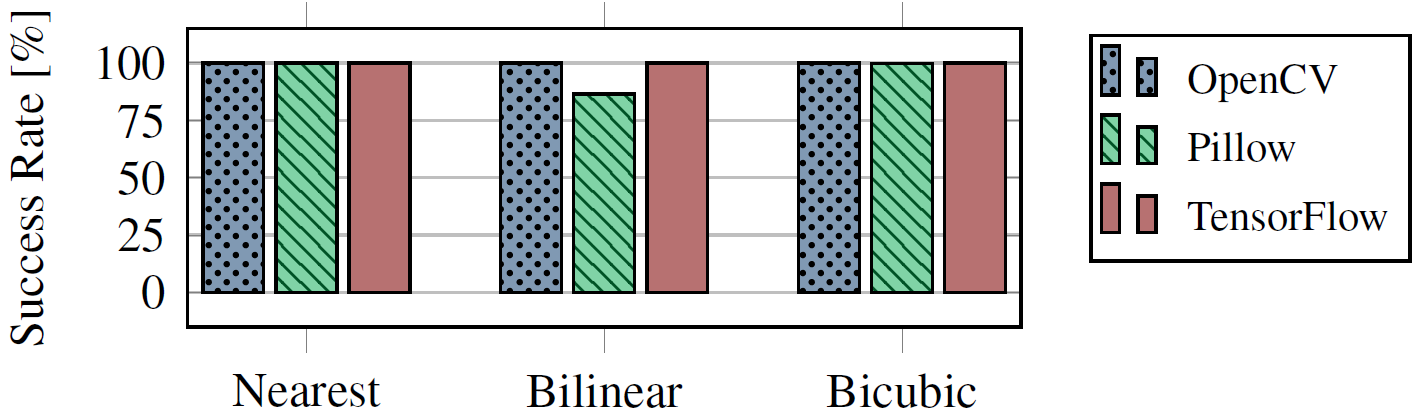
\includegraphics[width=\linewidth]{img/resO1.png}
  \caption{\DIFaddFL{Evaluation results in terms of $\boldsymbol{O_1}$. The diagram shows the success rate for the different algorithms nearest-neighbor, bilinear and bicubic of the frameworks OpenCV, Pillow and Tensorflow \mbox{%DIFAUXCMD
\cite{imgscale}}\hspace{0pt}%DIFAUXCMD
.}}
  \Description{}
  \label{fig:results_algos_o1}
\end{figure}

\begin{figure}[h]
  \centering
  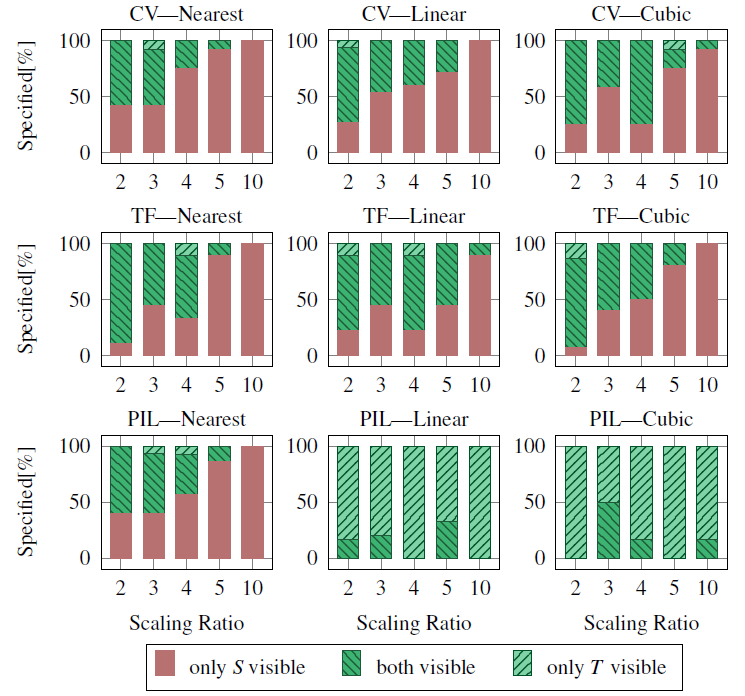
\includegraphics[width=\linewidth]{img/resUserStudy.png}
  \caption{\DIFaddFL{Evaluation results in terms of $\boldsymbol{O_2}$. The diagram shows the user study results of Quiring et al. in respect to the algorithms nearest-neighbor, bilinear and bicubic of the frameworks OpenCV, Pillow and Tensorflow \mbox{%DIFAUXCMD
\cite{imgscale}}\hspace{0pt}%DIFAUXCMD
.}}
  \Description{}
  \label{fig:results_algos_o2}
\end{figure}
\DIFaddend 

\subsubsection{Robustness of Defensive Strategies}
To analyze if their suggested defensive strategies\DIFaddbegin \DIFadd{, namely the median based and the random filter based recovering strategy (\ref{sec:median_filter}), }\DIFaddend effectively can prevent the image-scaling attack, Quiring et al. evaluated them for all scenarios in which the attacks succeeded without any defenses.
Their results show, that the suggested defense successfully can mitigate the achievement of $\boldsymbol{O_1}$ for \DIFdelbegin \DIFdel{all cases.
Furthermore }\DIFdelend \DIFaddbegin \DIFadd{most cases.
Therefore, }\DIFaddend they evaluated the \DIFaddbegin \DIFadd{success rate of reconstructing the source image $S$ by predicting the reconstructed images with the VGG19 model.
An image is considered to be correctly reconstructed, if the the model prediction matches the prediction of the original source image $S$.
Besides evaluating the reconstructed images that were affected by an attack, Quiring et al. investigated the }\DIFaddend effect of their defense on images that were not corrupted by an attacker.
\DIFdelbegin \DIFdel{They showed, that }\DIFdelend \DIFaddbegin \DIFadd{The results of their evaluation are shown in figure~\ref{fig:defRes}.
For }\DIFaddend the median based recovering strategy \DIFdelbegin \DIFdel{could be applied with minor losses in prediction accuracy, while }\DIFdelend \DIFaddbegin \DIFadd{a success rate of nearly 100\% for all evaluated algorithms could be achieved.
However, the results for }\DIFaddend the random filter based strategy \DIFdelbegin \DIFdel{affected the prediction accuracy stronger}\DIFdelend \DIFaddbegin \DIFadd{are worse.
The worst reported result is a success rate of only 88.1\% for the nearest-neighbor algorithm of the Pillow framework}\DIFaddend .

\DIFaddbegin \begin{figure}[h]
  \centering
  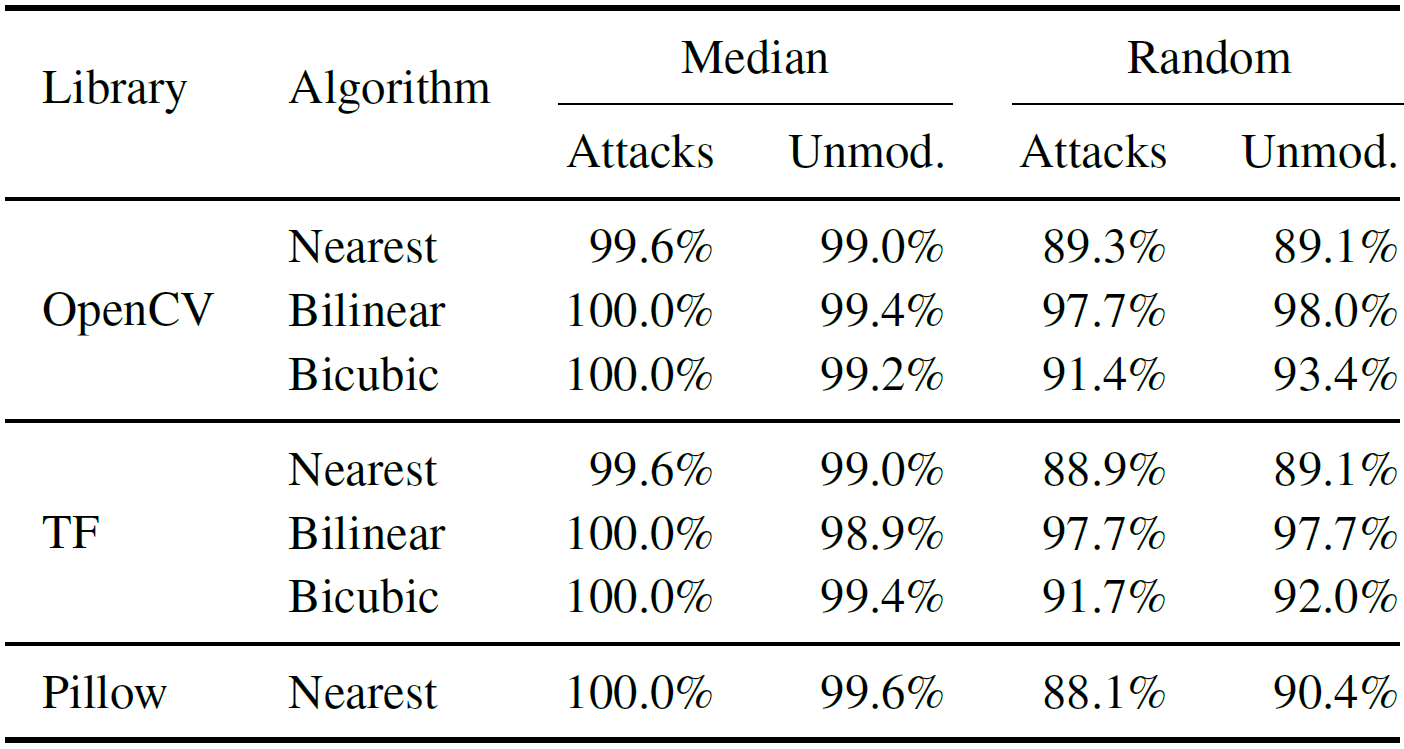
\includegraphics[width=\linewidth]{img/defRes.png}
  \caption{\DIFaddFL{Evaluation results of the defensive strategies. The table shows the rate of correctly reconstructed images in respect to the algorithms nearest-neighbor, bilinear and bicubic of the frameworks OpenCV, Pillow and Tensorflow. 
  		The column ``Unmod.`` shows the prediction accuracy of the evaluated model of images that were not attacked, but still modified by the defensive strategy \mbox{%DIFAUXCMD
\cite{imgscale}}\hspace{0pt}%DIFAUXCMD
.}}
  \Description{}
  \label{fig:defRes}
\end{figure}

\DIFaddend \subsection{Image-Scaling Attacks at Train Time}
This section covers the kind of attack that is described in section \ref{sec:traintimeatt}.

\subsubsection{Setup \& Evaluation}
The setup, chosen by Quiring et al.\cite{imgscalepoison} is as follows:
For their evaluation, they use the model of Carlini \& Wagner \cite{7958570} along with the CIFAR-10 \DIFdelbegin \DIFdel{dataset }\DIFdelend \DIFaddbegin \DIFadd{data set }\DIFaddend \cite{cifar}.
In order to enable an image-scaling attack, they upscale the images from the CIFAR-10 \DIFdelbegin \DIFdel{dataset }\DIFdelend \DIFaddbegin \DIFadd{data set }\DIFaddend to a size of $256 \times 256$.
Note that the used model requires inputs of size $32 \times 32$.
As attack strategy, the strong strategy is applied.
The used downscaling \DIFdelbegin \DIFdel{algorithms }\DIFdelend \DIFaddbegin \DIFadd{algorithm }\DIFaddend is the bilinear algorithm with the implementation of TensorFlow.

\subsubsection{Enforced Backdoor Attack}
To perform the attack, Quiring et al. embed a filled black square in the lower left corner of the training images, following the concept explained in section \ref{sec:traintimeatt}.
In order to assess their results, they compared them to a baseline that represents the results of the backdoor attack without using the image-scaling attack.
It could be shown that their attack succeeded in case that at least 5\% \DIFdelbegin \DIFdel{if }\DIFdelend \DIFaddbegin \DIFadd{of }\DIFaddend the training data were changed while the visible traces on the manipulated data hardly could be detected by a human observer.
Furthermore no drawbacks in comparison to the basic backdoor attack could be observed \DIFaddbegin \DIFadd{(see figure~\ref{fig:resBadNet})}\DIFaddend .
Thus Quiring et al. proved that a backdoor attack \DIFdelbegin \DIFdel{can }\DIFdelend \DIFaddbegin \DIFadd{might }\DIFaddend benefit from an image-scaling attack in a way, that it \DIFdelbegin \DIFdel{provides stealthiness to the attack. }\DIFdelend \DIFaddbegin \DIFadd{hides the backdoor pattern.
For more detailed information we would like to refer to the paper of Quiring et al. \mbox{%DIFAUXCMD
\cite{imgscalepoison}
}\hspace{0pt}%DIFAUXCMD
}

\begin{figure}[h]
  \centering
  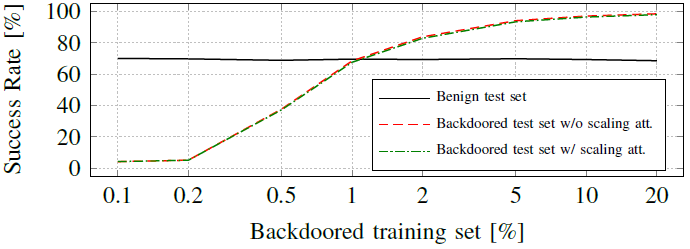
\includegraphics[width=\linewidth]{img/resBadNet.png}
  \caption{\DIFaddFL{Evaluation results of the image-scaling enforced backdoor attack of Quiring et al. The diagram shows the success rate of the poisoning attacks with and without the combination with the image-scaling attack \mbox{%DIFAUXCMD
\cite{imgscalepoison}}\hspace{0pt}%DIFAUXCMD
}}
  \Description{}
  \label{fig:resBadNet}
\end{figure}
\DIFaddend 

\subsubsection{Detection}
To evaluate the visible traces of their image-scaling enforced backdoor attack \DIFaddbegin \DIFadd{on the attack image $A$}\DIFaddend , they used the detection methods, explained in section \ref{sec:detection}.
Since the backdoor pattern is widely spread on the attack image $A$ and only covers a small region on the down-scaled image $scale(A)$ the resulting histograms of a $A$ - $scale(A)$ do not differ enough to detect any obvious dissimilarities.
Thus the detection mechanisms fail for this kind of attack.
Note that Quiring et al. did not evaluate any defensive strategies for this scenario. 

\subsection{Further Experiments}
\DIFaddbegin \label{sec:fexp}
\DIFaddend In order to evaluate some of the results from Quiring et al. this section presents a few, rudimentary results of further experiments that are based on the open source code, provided by Quiring et al.

Since image-scaling attacks as well as their detection and defenses are meant to be independent from any potentially attacked model, the presented experiments rather focus on the image processing than on the relation to any model.
Thus an attack is considered to be successful in terms of $\boldsymbol{O_1}$, if the down-scaled image visually is perceptible as the intended class instance by a human (instead of a machine learning model).
$\boldsymbol{O_2}$ can be evaluated using the PSNR score.

The followings \DIFdelbegin \DIFdel{experiments }\DIFdelend \DIFaddbegin \DIFadd{experiment scenarios }\DIFaddend were done for each four image pairs from private photos:
\DIFdelbegin \textbf{\DIFdel{a)}} %DIFAUXCMD
\DIFdelend \DIFaddbegin 

\begin{itemize}
\item[\textbf{a)}] \DIFaddend The image-scaling attack is applied on the images without any defensive mechanisms. 
\DIFdelbegin \textbf{\DIFdel{b)}} %DIFAUXCMD
\DIFdelend \DIFaddbegin \item[\textbf{b)}] \DIFaddend The image-scaling attack is applied using the median filter defense.
\DIFdelbegin \textbf{\DIFdel{c)}} %DIFAUXCMD
\DIFdelend \DIFaddbegin \item[\textbf{c)}] \DIFaddend The image-scaling attack is applied without any defenses to hide a backdoor pattern that can be used for a poisoning attack.
\DIFaddbegin \end{itemize}

\DIFaddend The used downscaling \DIFdelbegin \DIFdel{algorithms }\DIFdelend \DIFaddbegin \DIFadd{algorithm }\DIFaddend is the bilinear algorithm with the implementation of TensorFlow. 

\DIFdelbegin \DIFdel{All }\DIFdelend \DIFaddbegin \DIFadd{One example of the evaluation is shown in figure~\ref{fig:ev1}.
Additional results are shown in the appendix~\ref{sec:app}.
In the following the results of the different scenarios are presented:
}

\smallbreak

\textit{\DIFadd{Image-Scaling Attack without defense:}}
\DIFadd{Objective $\boldsymbol{O_1}$ is achieved for every image pair.
Even without any model predictions, it is clearly visible that every output image $D$ is similar to its corresponding target image $T$.
Considering the chosen threshold of a PSNR score $\geq$ 15dB, the objective $\boldsymbol{O_2}$ is achieved for 3 out of 4 image pairs by a lot.
Even though the remaining image pair achieves $\boldsymbol{O_2}$ with a PSNR score of 19.72dB, the corresponding attack image clearly can be detected by human observation (see figure~\ref{fig:results2}).
}

\smallbreak

\textit{\DIFadd{Image-Scaling Attack with defense:}}
\DIFadd{For all image pairs, the image-scaling attack fails in terms of objective $\boldsymbol{O_1}$.
As shown in figure~\ref{fig:ev1} and~\ref{fig:results2}, every resulting output image $D$ is clearly similar to its corresponding source image $S$.
}

\smallbreak

\textit{\DIFadd{Enforced Backdoor Attack:}}
\DIFadd{As the qualitative results in figure~\ref{fig:ev1} and~\ref{fig:results2} show, the applied backdoor pattern can be hidden within the attack image $A$, while it is still visible on the resulting output image $D$.
Note that the reported PSNR scores are even higher than the scores reported for scenario }\textbf{\DIFadd{a)}}\DIFadd{.
Thus the scenario can be considered to be successful in terms of $\boldsymbol{O_1}$ and  $\boldsymbol{O_2}$ .
}

\smallbreak

\DIFadd{Overall the }\DIFaddend experimental results showed to be consistent with the insights of Quiring et al. \DIFdelbegin \DIFdel{and thus }\DIFdelend \DIFaddbegin \DIFadd{so that }\DIFaddend their conclusions can be confirmed \DIFdelbegin \DIFdel{.
Note that these examples }\DIFdelend \DIFaddbegin \DIFadd{for the evaluated scenarios.
However, the aforementioned experiments only cover a small scope of potential evaluation scenarios and }\DIFaddend are based on a very small set of images\DIFdelbegin \DIFdel{and thus }\DIFdelend \DIFaddbegin \DIFadd{. 
Thus they }\DIFaddend are not empirically representative.
\DIFdelbegin \DIFdel{A qualitative example that shows how an image of myself can be turned into an image of a friend of mine, is shown in \ref{fig:results}.
}\DIFdelend 

\begin{figure}[h]
  \centering
  \DIFdelbeginFL %DIFDELCMD < 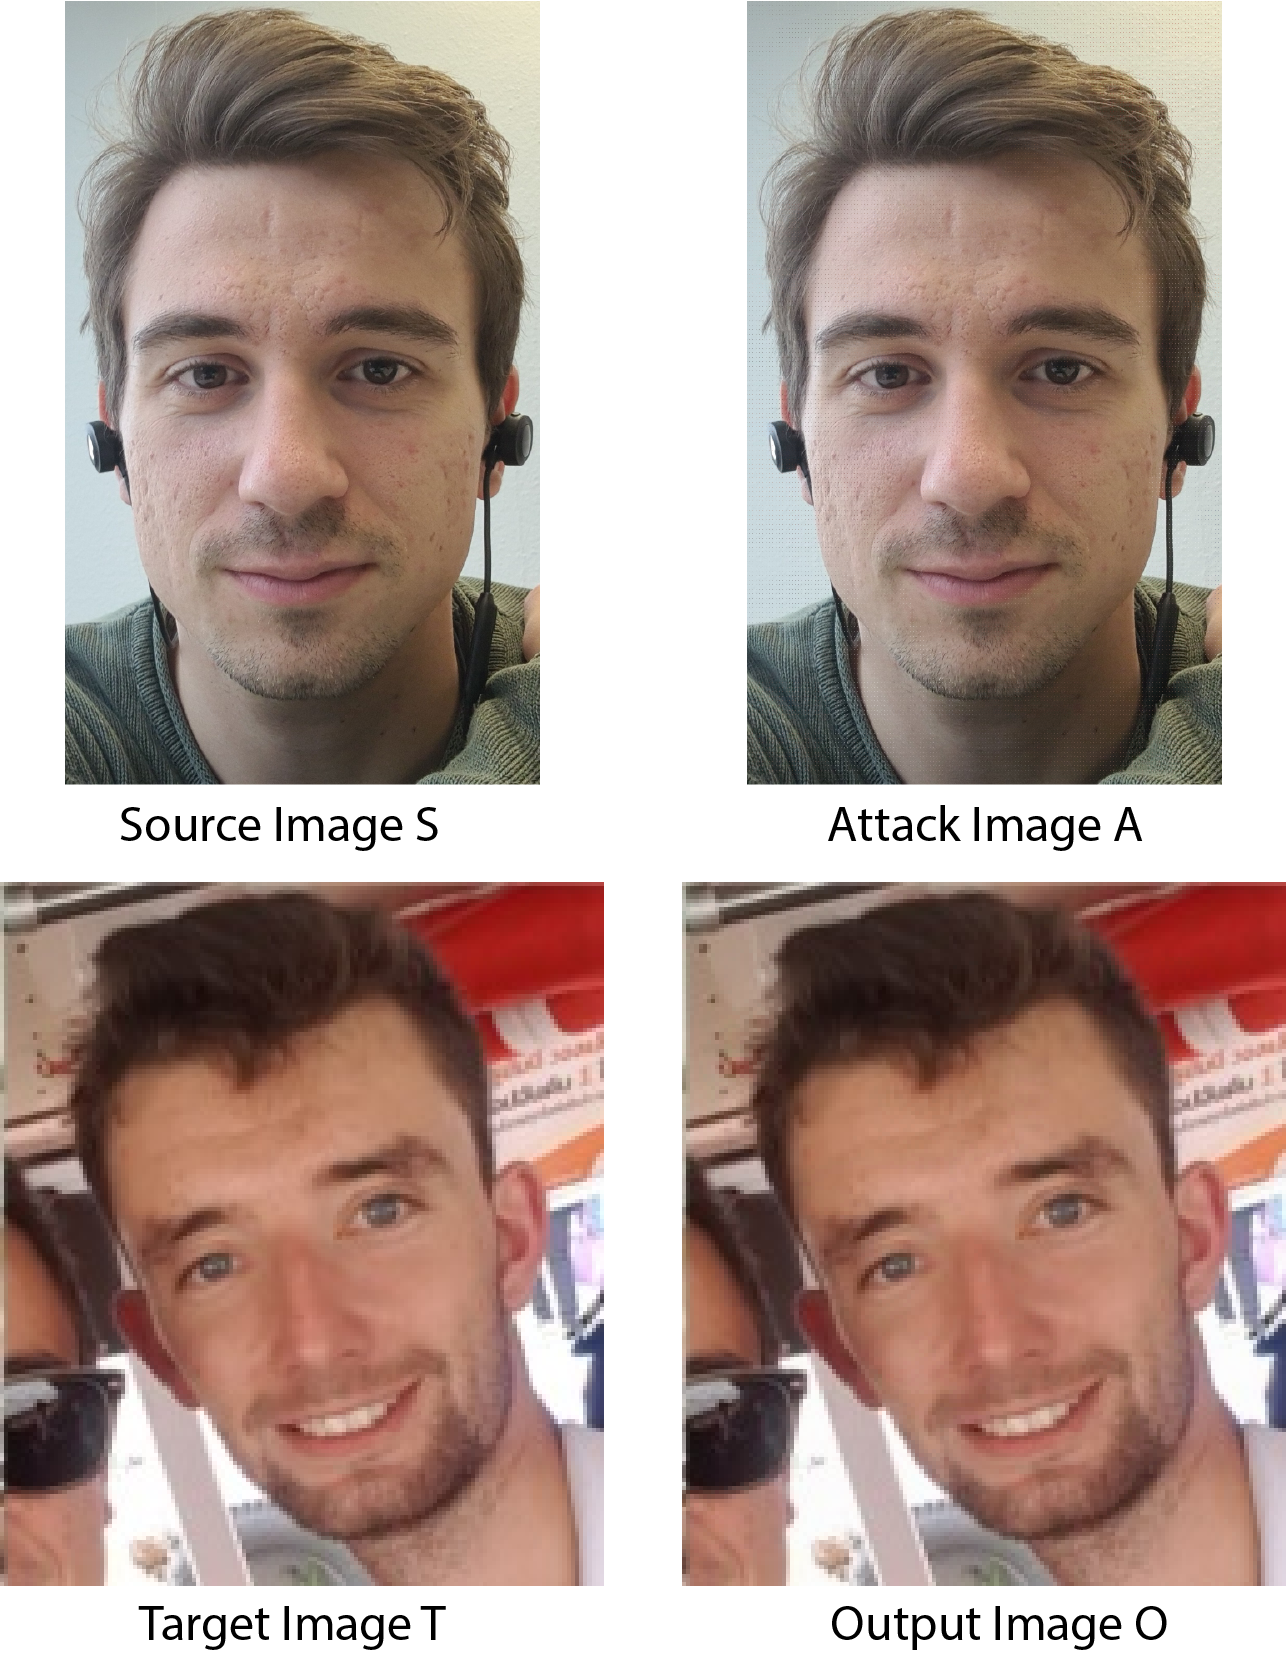
\includegraphics[width=\linewidth]{img/attackExample.png}
%DIFDELCMD <   %%%
\DIFdelendFL \DIFaddbeginFL 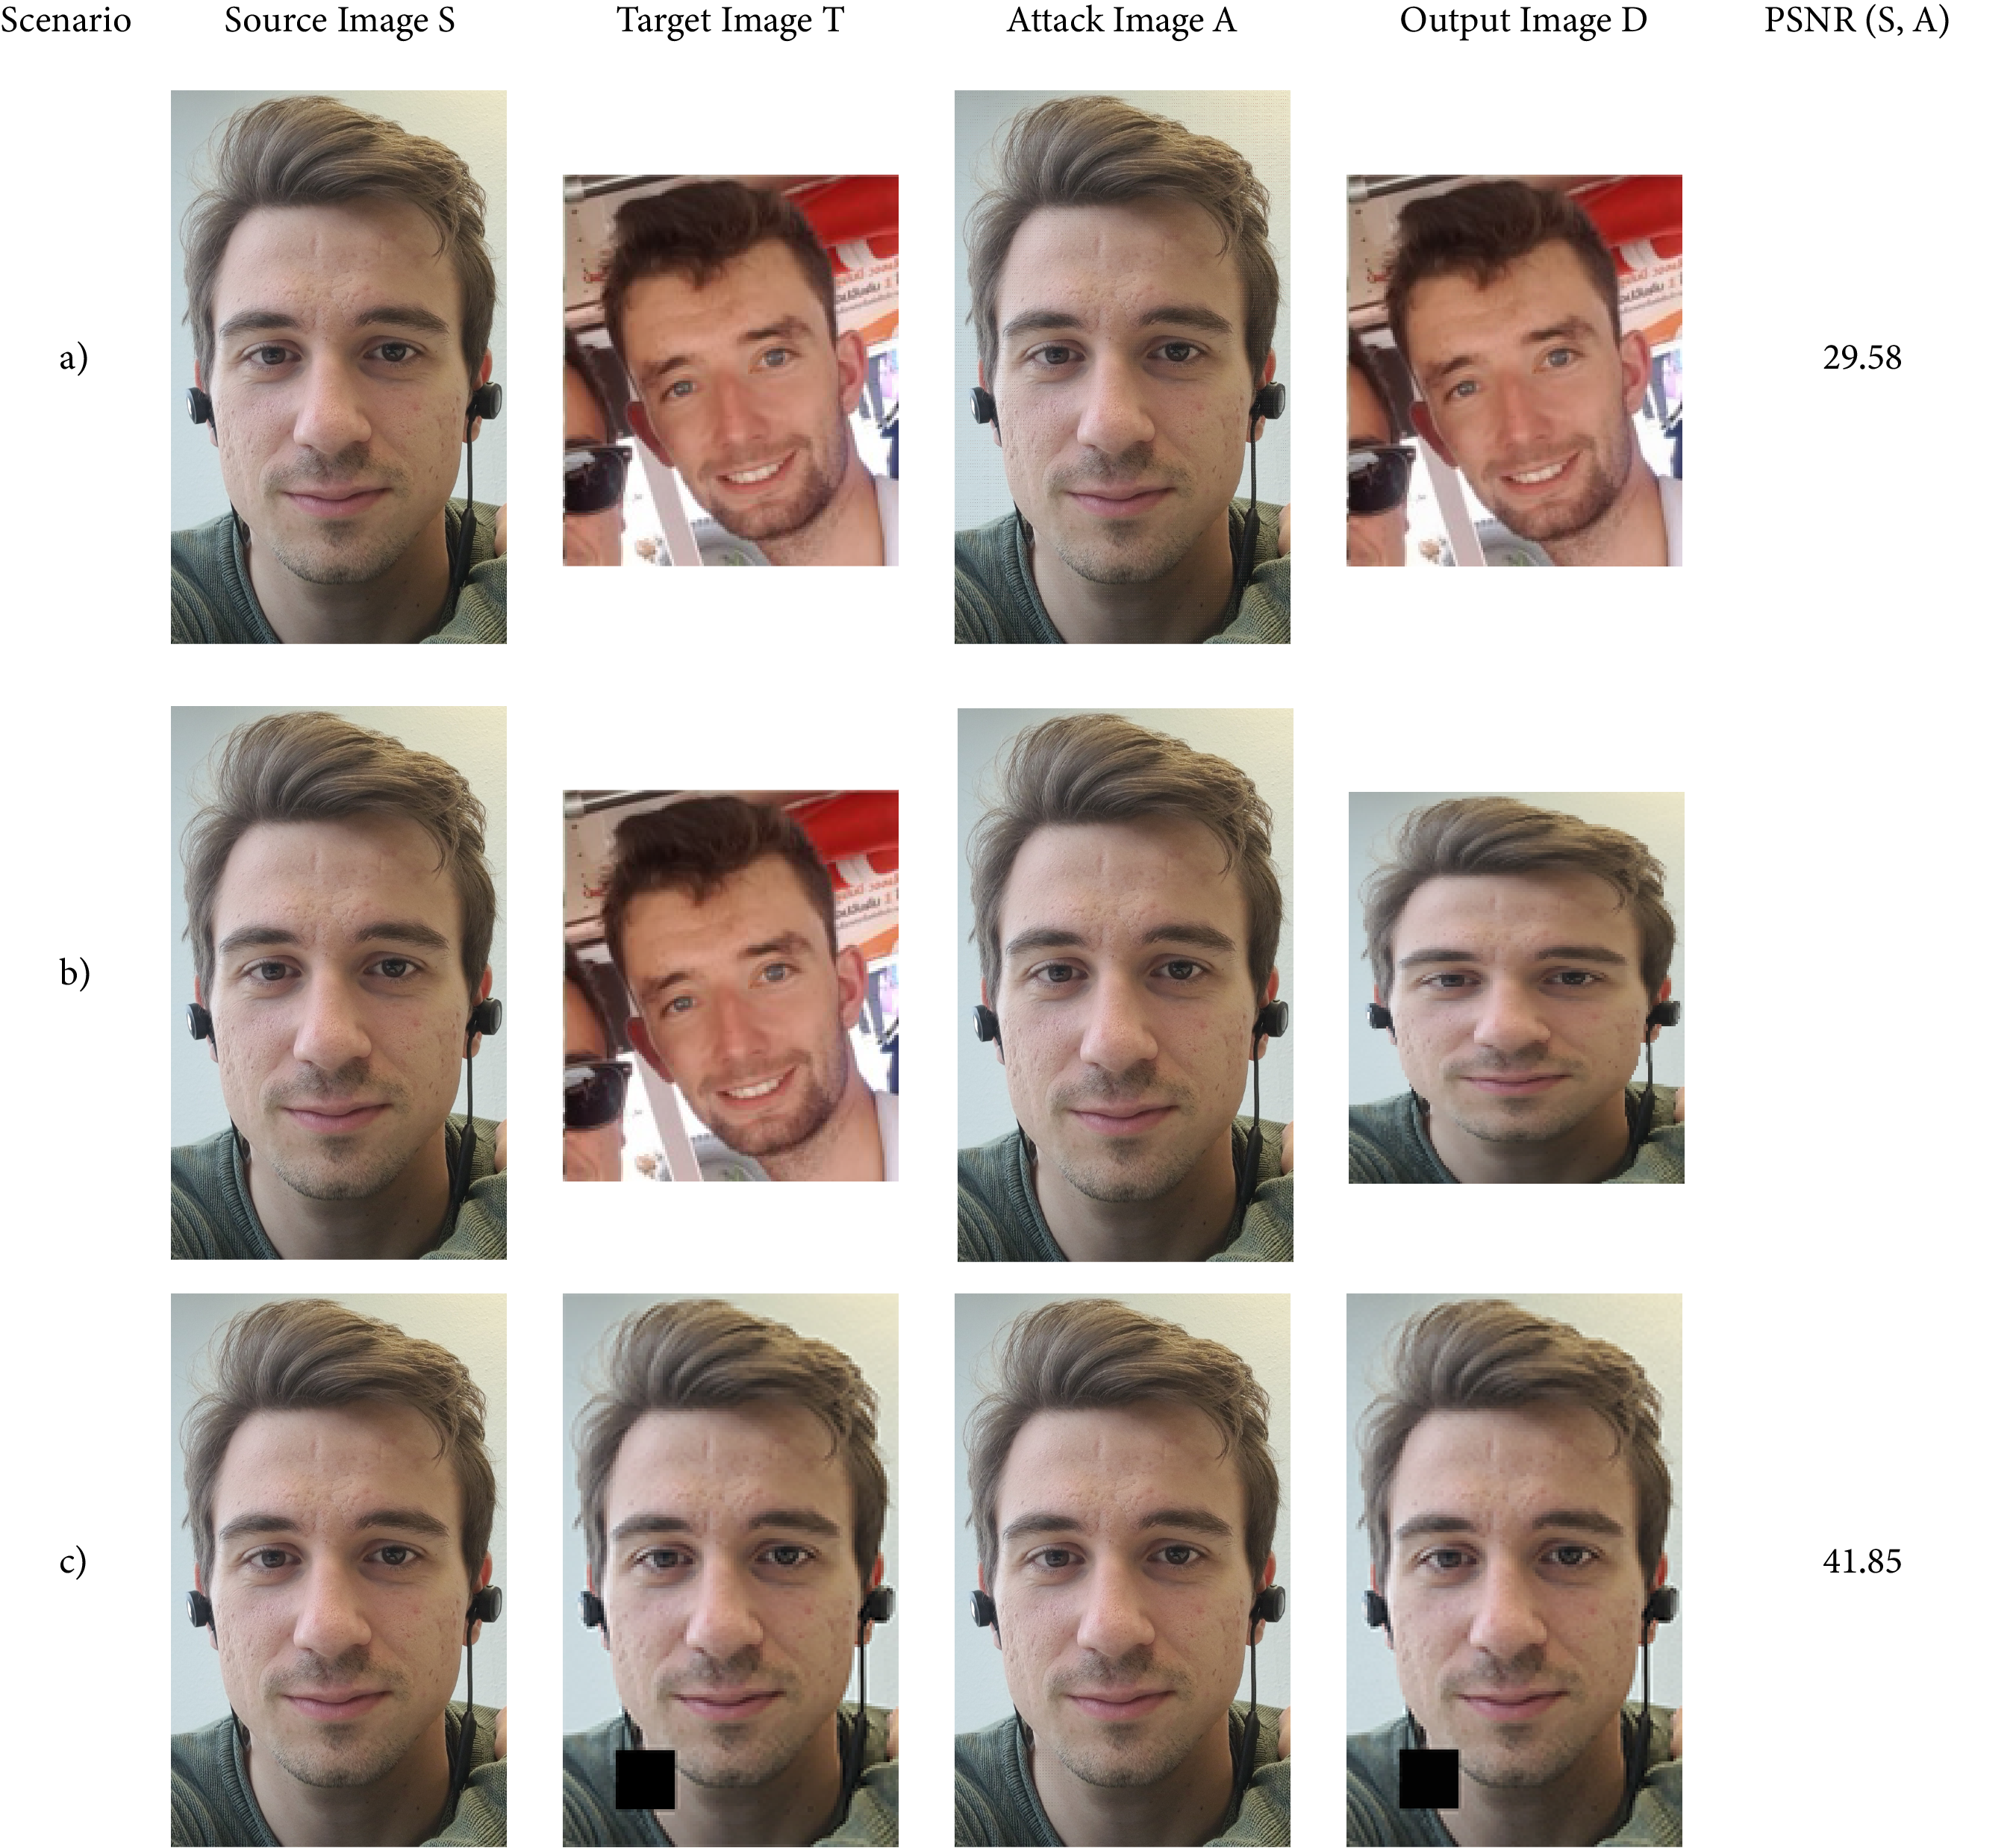
\includegraphics[width=\linewidth]{img/eval1.png}
  \DIFaddendFL \caption{\DIFdelbeginFL \DIFdelFL{Example }\DIFdelendFL \DIFaddbeginFL \DIFaddFL{Evaluation results }\DIFaddendFL of \DIFdelbeginFL \DIFdelFL{an Image-Scaling Attack on an Image }\DIFdelendFL \DIFaddbeginFL \DIFaddFL{one image pair }\DIFaddendFL of \DIFdelbeginFL \DIFdelFL{myself}\DIFdelendFL \DIFaddbeginFL \DIFaddFL{the scenarios }\textbf{\DIFaddFL{a)}}\DIFaddFL{, }\textbf{\DIFaddFL{b)}} \DIFaddFL{and }\textbf{\DIFaddFL{c)}}\DIFaddFL{. For each scenario, the images $S$, $T$, $A$ and $D$, as well as the PSNR score are shown. 
  		Note that the attack image $A$ of scenario }\textbf{\DIFaddFL{b)}} \DIFaddFL{is the attack image after being reconstructed by the median filter based recovering strategy. Furthermore no PSNR score is reported for this scenario, since the attack fails in terms of $\boldsymbol{O_1}$}\DIFaddendFL .\DIFdelbeginFL \DIFdelFL{$PSNR(S, A) = 29.58$}\DIFdelendFL }
  \Description{}
  \DIFdelbeginFL %DIFDELCMD < \label{fig:results}
%DIFDELCMD < %%%
\DIFdelendFL \DIFaddbeginFL \label{fig:ev1}
\DIFaddendFL \end{figure}

\section{Conclusion}
\DIFdelbegin \DIFdel{This section recaps the presented works of Quiring et al. and Xiao et al. and briefly discusses the key conclusions that can be drawn.
}%DIFDELCMD < 

%DIFDELCMD < %%%
\DIFdelend In this work the new image-scaling attack, its basic concept and the root-cause that enables the attack were presented.
Furthermore several ways to use such an attack to manipulate machine learning based image processing applications as well as proper detection and defense strategies were shown.
The efficacy of the suggested defenses as well as the successful realization of an image-scaling attack enforced poisoning attack were proven by the presented experiments of Quiring et al. and further supported by additional experiments.

First of all it can be seen, that the new image-scaling attack enables new ways for attackers to manipulate machine learning based applications.
Two major benefits of this new attack strategy is the fact, that it can be applied independent from the attacked model and the required algorithms can be processed automatically and efficiently.
Another benefit is the stealthiness that is provided by the attack.

However, since the attack is applied at the preprocessing stage of a machine learning pipeline, it is way easier to analyze, than attacks that directly are applied to a model.
Hence there could be developed simple detection and defensive methods that can mitigate an image-scaling attack.
Especially the suggested defense by Quiring et al. proved to be successful for the evaluated attack scenarios at test time.
Since poisoning attacks are mostly based on the manipulation of the training data, it is questionable, if these defenses realistically can be applied in a poisoning attack scenario. 

Overall the work of Quiring et al. and Xiao et al. showed that there exists a realistic risk of image-scaling attacks for security critical applications, if no proper defenses are applied.
Furthermore it is shown that the preprocessing stage of machine learning pipelines is as vulnerable as the training stage and the test stage, even if defensive strategies might easier to be identified and applied.
However, \DIFdelbegin \DIFdel{currently there don't exist any works }\DIFdelend \DIFaddbegin \DIFadd{on our research we didn't find any other works within the domain of computer vision }\DIFaddend about attacks on other preprocessing steps than image-scaling.
This might be an \DIFdelbegin \DIFdel{interestin }\DIFdelend \DIFaddbegin \DIFadd{interesting }\DIFaddend field for future research.

%%
%% The next two lines define the bibliography style to be used, and
%% the bibliography file.
\bibliographystyle{ACM-Reference-Format}
\bibliography{base}
\DIFaddbegin 

\newpage
\appendix

\section{\DIFadd{Additional Evaluation Results}}
\label{sec:app}

\begin{figure}[h]
  \centering
  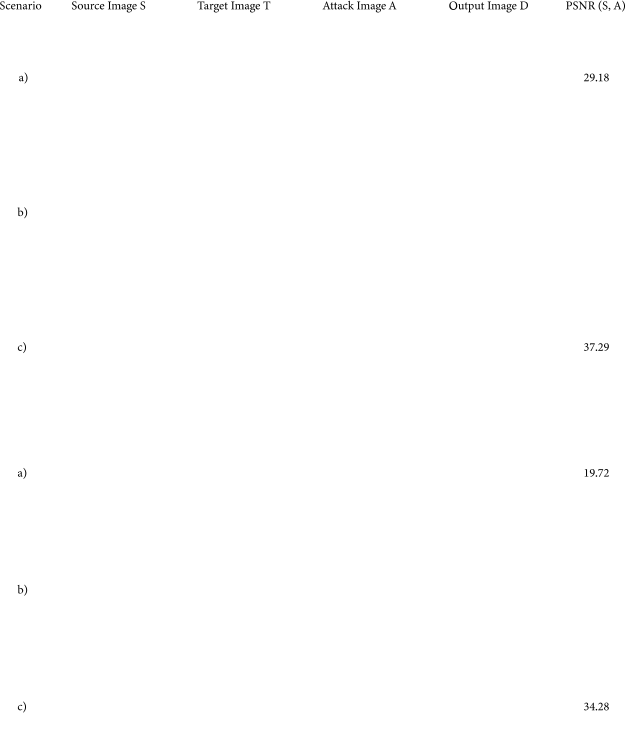
\includegraphics[width=\linewidth]{img/eval2.png}
  \caption{\DIFaddFL{Additional evaluation results of the scenarios }\textbf{\DIFaddFL{a)}}\DIFaddFL{, }\textbf{\DIFaddFL{b)}} \DIFaddFL{and }\textbf{\DIFaddFL{c)}} \DIFaddFL{mentioned in section~\ref{sec:fexp}. For each scenario, the images $S$, $T$, $A$ and $D$, as well as the PSNR score are shown. 
  		Note that the attack image $A$ of scenario }\textbf{\DIFaddFL{b)}} \DIFaddFL{is the attack image after being reconstructed by the median filter based recovering strategy. Furthermore no PSNR score is reported for this scenario, since the attack fails in terms of $\boldsymbol{O_1}$.}}
  \Description{}
  \label{fig:results2}
\end{figure}
\DIFaddend 

\end{document}
\endinput
%%
%% End of file `sample-sigconf.tex'.
